\documentclass[a4paper,12pt,twoside,openright]{mwrep}
%
%
\usepackage{polski}
\usepackage{helvet}
\usepackage[T1]{fontenc}
\usepackage{anyfontsize}
\usepackage[utf8]{inputenc}
\usepackage[pdftex]{graphicx}
\usepackage{tabularx}
\usepackage{array}
%\usepackage{subfigure}
\usepackage{amsfonts}
\usepackage{verbatim}
\usepackage{indentfirst}
\usepackage[pdftex]{hyperref}
\usepackage[none]{hyphenat}
\usepackage{float}
\usepackage[title,titletoc]{appendix}

% usun kropki po rzymskich
\usepackage{caption}
\captionsetup[table]{labelsep=space}
\captionsetup[figure]{labelsep=period}

% interlinia
\linespread{1.3} % 1 - pojedyncza, 1.3 - poltora, 1.6 - podwojna

% aby nie bylo kropek w spisie treści 
%\makeatletter
%\renewcommand\@dotsep{200}

% rozdziały, sekcje niewidoczne w spisie treści
\newcommand{\nocontentsline}[3]{}
\newcommand{\tocless}[2]{\bgroup\let\addcontentsline=\nocontentsline#1{#2}\egroup}
%
% przykład:
% w treści dokumentu wstaw
% \tocless\section{Rozdział niewidoczny w spisie tresci}

\renewcommand*\thetable{\Roman{table}}


%pakiet anysize - papersize marginsize

% rozmaite polecenia pomocnicze
% gdzie rysunki?
\newcommand{\ImgPath}{.}

% oznaczenie rzeczy do zrobienia/poprawienia
\newcommand{\TODO}{\textbf{TODO}}


% wyroznienie slow kluczowych
\newcommand{\tech}{\texttt}

% na oprawe (1.0cm - 0.7cm)*2 = 0.6cm
% na oprawe (1.1cm - 0.7cm)*2 = 0.8cm
%  oddsidemargin lewy margines na nieparzystych stronach
% evensidemargin lewy margines na parzystych stronach
%\def\oprawa{1.05cm}
%\addtolength{\oddsidemargin}{\oprawa}
%\addtolength{\evensidemargin}{-\oprawa}

%\geometry{tmargin=2cm, bmargin=1.5cm, lmargin=3.5cm, rmargin=2cm}

%marginesy jakie są każdy widzi
\usepackage[tmargin=2cm, bmargin=1.8cm, lmargin=3.5cm, rmargin=2.0cm]{geometry}

% table span multirows
\usepackage{multirow}
\usepackage{enumitem}	% enumitem.pdf
\setlist{listparindent=\parindent, parsep=\parskip} % potrzebuje enumitem

% aby itemize były - a nie *
\renewcommand\labelitemi{--}

%%%%%%%%%%%%%%% Dodatkowe Pakiety %%%%%%%%%%%%%%%%%
%\usepackage{prmag2017}   % definiuje komendy opiekun, nrindeksu, rodzaj pracy, ...


%%%%%%%%%%%%%%% Strona Tytułowa %%%%%%%%%%%%%%%%%
% To trzeba wypelnic swoimi danymi
\title{Wpływ pracy zawodowej w ponadnormatywnym wymiarze czasu pracy na życie osobiste pielęgniarek i pielęgniarzy}

% autor
\author{Małgorzata Ługin-Dąbrowska}
	
%	\nrindeksu{3942}

%	\opiekun{dr n. med. Marta Gawlik}

%	\terminwykonania{1 maja 2022} % data na oświadczeniu o samodzielności

%	\rok{2022}

%\Pielęgniarkom przyszłym i obecnym
%\podziekowania{\noindent
{\Large Podziękowania}
\bigskip

Dziękujemy bardzo serdecznie wszystkim, a w szczególności Rodzinom i~Unii Europejskiej...

\bigskip

{\raggedleft
Zdolny Student i Pracowity Kolega

}

}

%	\miasto{Legnica}

%	\uczelnia{Wyższa Szkoła Medyczna}

%	\wydzial{WYDZIAŁ PIELĘGNIARSTWA}

%	\kierunekstudiow{PIELĘGNIARSTWO}

% domyslnie praca jest inzynierska, ale po odkomentowaniu ponizszej linii zrobi sie magisterska
%	\pracamagisterska
%%% koniec od P.W

%\streszczenia{
%  \newpage
\begin{center}
\large \bf
TYTUŁ PRACY DYPLOMOWEJ
\end{center}

\section*{Streszczenie}
Praca składa się z krótkiego wstępu jasno i
wyczerpująco opisującego oraz uzasadniającego cel pracy, trzech rozdziałów (2-4)
zawierających opis istniejących podobnych
rozwiązań, komponentów rozpatrywanychjako kandydaci do
tworzonego systemu i wreszcie zagadnień wydajności wirtualnych
rozwiązań. Piąty rozdział to opis  środowiska obejmujący opis konfiguracji
środowiska oraz przykładowe ćwiczenia laboratoryjne. Ostatni
rozdział pracy to opis możliwości dalszego
rozwoju projektu. 

\bigskip
{\noindent\bf Słowa kluczowe:} praca dyplomowa, LaTeX, jakość

\vskip 2cm


\begin{center}
\large \bf
THESIS TITLE
\end{center}

\section*{Abstract}
This thesis presents a novel way of using a novel algorithm to solve complex
problems of filter design. In the first chapter the fundamentals of filter design
are presented. The second chapter describes an original algorithm invented by the
authors. Is is based on evolution strategy, but uses an original method of filter
description similar to artificial neural network. In the third chapter the implementation
of the algorithm in C programming language is presented. The fifth chapter contains results
of tests which prove high efficiency and enormous accuracy of the program. Finally some
posibilities of further development of the invented algoriths are proposed.

\bigskip
{\noindent\bf Keywords:} thesis, LaTeX, quality

\vfill
%}

%uaktywnić specjalne komendy związane z tworzeniem indeksów.
%\makeindex

%modyfikacja odległości przed tyytułem rozdziału
\makeatletter
\SetSectionFormatting[breakbefore,wholewidth]{chapter}
        {33\p@}  %<-------------------- change this value (default is 56)
        {\FormatBlockHeading{\LARGE}}
        {24\p@}
\makeatother


\begin{document}
\sloppy
\maketitle

\newpage

\centerline{Pielęgniarkom przyszłym i obecnym}
%\newpage

\tableofcontents

%\printindex

\newpage
% Wykaz skrótów
\Large Wykaz skrótów
\normalsize

%\tocless\section{Wykaz skrótów}
%\section*{Wykaz skrótów}


\begin{table}[ht]
    
    \label{tab:index}
    %\begin{tabular}{*{2}{l}}
	\begin{tabular}{  l  l  }
	
    APA & (\textit{ang. American Psyhologic Association}) Amerykańskie Towarzystwo Psychologiczne \\
	
	CBOS & Centrum Badania Opinii Społecznej \\

	Dz. U. & Dziennik Ustaw \\

	EBM & (\textit{ang. Evidence-Based Medicine}) Medycyna Oparta na Faktach \\
	
	ICD -11& (\textit{ang. International Classification of Diseases 11th}) Międzynarodowa Klasyfikacja Chorób \\
	
	Komórki NK & (\textit{ang. Natural Killer}) komórki Naturalni Zabójcy - limfocyty \\

	MZ & Ministerstwo Zdrowia\\

	NIPIP & Naczelna Izba Pielęgniarek i Położnych\\

	OIPIP & Okręgowa Izba Pielęgniarek i Położnych\\

	POZ & Podstawowa Opieka Zdrowotna\\

	PTSD & (\textit{ang. Post-Traumatic Stress Disorder}) Zespół Stresu Pourazowego \\

	SOZ & System Ochrony Zdrowia\\
	
	UNICEF & Fundusz Narodów Zjednoczonych na rzecz Dzieci\\

	WHO & (\textit{ang. World Health Organization}) Światowa Organizacja Zdrowia \\
	
	WSM& Wyższa Szkoła Medyczna w Legnicy\\
     
     e-ZLA & elektroniczne zwolnienie lekarskie \\

	ZNPZ & Zespół Nietolerancji Pracy Zmianowej \\
	

	
	\end{tabular}
   

\end{table}





%-----------------
% Wstęp
%-----------------

\chapter*{Wstęp}

Pielęgniarstwo jest tak stare jak ludzkość. Zawsze ludziom towarzyszyły choroby i zawsze były osoby, które rozwiązywały problem na miarę własnych możliwości i na miarę czasów, w których żyły. Postęp naukowy i technologiczny, zmienił postrzeganie pielęgniarstwa z zawodu opiekuńczego, na zawód samodzielny - obejmujący pacjenta w integralności biopsychospołecznej. Pielęgniarstwo, w Polsce od 1996 roku jest autonomicznym zawodem \cite{konst97art17}. Jest także profesją zaufania publicznego, a pielęgniarki i pielęgniarze są chronieni prawnie, w trakcie wykonywania swoich obowiązków zawodowych jak funkcjonariusze publiczni \cite{art4uozp}.

Pielęgniarstwo, to obecnie dyscyplina naukowa dotycząca rozważań teoretycznych, badań in vitro, in vivo, które można wykorzystać w praktyce. Są to doniosłe osiągnięcia pielęgniarek i pielęgniarzy, którzy prowadzą badania na uczelniach, w klinikach, laboratoriach badawczych na całym świecie \cite{nursingresearch}.

Pielęgniarstwo to zaszczyt, prestiż, ale i wyzwanie. Ustawiczne kształcenie, wyrzeczenia w życiu osobistym, stres, traumatyzacja, trudne warunki pracy są dalekie od pojęcia dobrostanu.  Niepokojące zjawiska, które dotykają organizacji pielęgniarstwa, zwłaszcza konsekwencje zdrowotne, wynikające z pracy w ponadnormatywnym wymiarze, stanowią obszar zainteresowań tego opracowania.

Celem głównym niniejszej pracy jest określenie wpływu pracy zawodowej na życie osobiste pielęgniarek i pielęgniarzy. Cel ten przybliżyły cele szczegółowe, dotyczące godzenia ról społecznych, świadomości pielęgniarek i pielęgniarzy, na temat zagrożeń wynikających z pracy ponadnormatywnym czasie, poziomu satysfakcji zawodowej oraz oceny Systemu Opieki Zdrowotnej w zakresie promocji , przyszłości pielęgniarstwa.

Część teoretyczna przybliża: rozwój pielęgniarstwa na świecie i w Polsce, drogę do samodzielności zawodowej. Ukazuje dynamikę zmian w zakresie kompetencji i~uprawnień. Rozważania na temat pełnienia ról społecznych: zawodowej i rodzinnej, a~także na temat zdrowia i systemów wsparcia pielęgniarek i~pielęgniarzy. 

Część badawcza składa się z części metodologicznej opisuje metody, narzędzia i~techniki badawcze. Przedstawia organizację i przebieg badania, zastosowane metody analizy statystycznej i graficznie prezentowane dane i wyniki. W dalszej kolejności występują wnioski oraz dyskusja z innymi badaczami.

Ostatnia część zawiera streszczenie, słowa kluczowe w języku polskim i angielskim, spisy tabel oraz załączniki.




%-----------------
% Wpływ pracy zawodowej pielęgniarek i pielęgniarzy na życie osobiste
%-----------------
\chapter{Wpływ pracy zawodowej pielęgniarek i~pielęgniarzy na życie osobiste w świetle literatury przedmiotu}

Zawód pielęgniarki należy do najbardziej prestiżowych profesji na świecie. W~wydanym przez WHO i Międzynarodową Radę Pielęgniarek raporcie o~stanie światowego pielęgniarstwa w roku 2020, podkreśla się szczególne znaczenie pielęgniarstwa, w każdym systemie ochrony zdrowia. Pielęgniarki pełnią kluczową rolę w sytuacji światowego zagrożenia zdrowotnego \cite{who}.  Również w Polsce coroczne rankingi najbardziej szanowanych zawodów, umieszczają tę grupę zawodową na~wysokich pozycjach \cite{rap}. Mimo tego, od lat, obserwuje się znaczną dysproporcję między powszechną opinią o szacunku, a kojarzeniem zawodu z niskim wynagrodzeniem, ciężką pracą fizyczną i umysłową oraz nieustannymi wyrzeczeniami w życiu osobistym. Fenomen pogłębia fakt, iż pielęgniarki w większości, nie żałują wyboru zawodu, podkreślają, że daje  im wiele satysfakcji.

  %-----------------
  % Historyczne uwarunkowania samodzielności zawodowej.
  %-----------------
\section{Historyczne uwarunkowania samodzielności zawodowej}
Pielęgniarstwo ewaluowało na przestrzeni wieków, od spontanicznego odruchu serca, do autonomii wysokiego poziomu. Już w starożytności, nad cierpiącymi, czuwały osoby, wykonujące czynności pielęgnacyjne. Istnieją źródła historyczne, dotyczące organizacji opieki pielęgnacyjnej w starożytnych Indiach, Rzymie, Chinach, Japonii czy Grecji. Choć początkowo role te pełnili mężczyźni, to z czasem zawód stał się domeną kobiet \cite{zro}. Od czasów średniowiecza pielęgnowaniem chorych zajmowały się siostry zakonne. Tradycyjne zwracanie się do pielęgniarek ,,siostro”, tam ma, swój początek. Przez wiele wieków pielęgniarki, kojarzono ze złą reputacją \cite{tlo}. Fakt ten, związany był z zatrudnianiem do pielęgnowania chorych  osób z marginesu społecznego. Dopiero Florence Nightingale w połowie XIX wieku  pokonując liczne przeszkody, otworzyła szkołę dla pielęgniarek. Główny nacisk oprócz typowych umiejętności pielęgniarskich położono, na nienaganne zachowanie w pracy i poza nią. Jej działalność na rzecz podniesienia prestiżu zawodu, jest niepodważalna  \cite{flo}. Wychowała wiele pokoleń pielęgniarek. Jej uczennice niosły kaganek zmian, nawet na inne kontynenty. Przykładem może być Linda'e Richards, znana jako pierwsza wyszkolona pielęgniarka USA, która promowała pielęgniarstwo, również w Japonii \cite{linda}.

Niezwykle istotne, dla przyszłości światowego pielęgniarstwa, było utworzenie w Stanach Zjednoczonych Ameryki, na przełomie wieków, Międzynarodowej Rady Pielęgniarek \cite{rada}. Organizacji zrzeszającej profesjonalistów, ściśle współpracującej z~takimi instytucjami jak WHO, Czerwony Krzyż czy UNICEF. Choć pielęgniarki polskie, włączone zostały do jej struktur, dopiero w 1948 roku, czynnie uczestniczyły w licznych projektach, dotyczących zdrowia i współpracy między tymi organizacjami.

\textit{W końcu nadszedł ten moment, w historii naszego zawodu, gdzie z poświęcenia i miłości bliźniego, przyszedł czas pielęgniarstwa zawodowego, opartego na wiedzy naukowej}. Cytowane słowa, wybitnej pielęgniarki i nauczycielki Marii Minczewskiej, podkreślają znaczenie zawodu, u którego podstawy, leży  ochrona najważniejszych wartości ludzkich – życia i zdrowia.  Co zawarte jest w postulatach, takich ikon pielęgniarstwa jak Dorota Orem, Virginia Henderson, Madelaine Leininger \cite{ikon}.

Nie bez znaczenia dla jakości pielęgniarstwa, są kamienie milowe pionierek zawodu z Kanady – kształcenie na uczelniach wyższych, idee promocji zdrowia.

Podwaliny pod profesjonalny, prestiżowy zawód były solidne. Wydawać by się mogło, że pielęgniarstwo w Polsce będzie się rozwijało, kwitło. Tak się nie stało. Na pewno wpływ na to miało położenie geopolityczne Polski. Sam fakt, że przez ponad wiek kraj był pod zaborami, nie sprzyjał budowaniu tej istotnej dla  Państwa dziedziny. Wojny Światowe przerywały działalność szkół pielęgniarskich: lwowskiej, krakowskiej, warszawskiej, jednak pielęgniarki ratowały i pielęgnowały ludzi pod auspicjami Czerwonego Krzyża.

Najbardziej znane i zasłużone pionierki polskiego pielęgniarstwa rozumiały, że~tylko nauka prowadzi do właściwego pełnienia tej roli zawodowej. Korzystały z~kursów prowadzonych przez pielęgniarki Czerwonego Krzyża  w Polsce, wyjeżdżały za granicę. Miały otwarte umysły i chętnie dzieliły się wiedzą, tworzyły szkoły, uczyły.  Wyznawały pogląd, że  \textit{żeby się dzielić, trzeba coś posiadać} \cite{ikonpol}. I to, czyniły ze swoim potencjałem intelektualnym i materialnym. Wśród wielu, koniecznie wymienić trzeba Hannę Chrzanowską, Zofię Szlenkier, Elżbietę Rabowską, Annę Rydlównę \cite{szkol}. Pamiętać należy, w jak trudnych czasach przyszło im żyć, z jakim poświeceniem zdobywały wiedzę nie zważając na ostracyzm, przeciwności losu. Powyższe przykłady powinny inspirować do świadomego wyboru i wykonywania zawodu pielęgniarki. Cieszy fakt, że~ich rola była doceniana nagrodami np. medalem Florence Nightingale, stypendiami np. Fundacji Rockefellera \cite{50}.

Po II Wojnie Światowej powrócono do kształcenia w zawodzie pielęgniarki. Nauka była prowadzona przez szkoły świeckie, pomaturalne. Istniały także krótkie ścieżki zawodowe. Powstała szkoła dla instruktorek pielęgniarstwa.

W kolejnych latach pojawiały się branżowe magazyny: \textit{Pielęgniarka Polska, Położna}, a w efekcie połączenia tych periodyków w 1958 roku, \textit{Pielęgniarka i Położna}. Wydawane przez Polskie Towarzystwo Pielęgniarskie \cite{czas}.

W 1968 roku Ministerstwo Zdrowia przyjęło zaproponowany system wyodrębnionych dziedzin pielęgniarskich. Tak pojawiło się pielęgniarstwo pediatryczne, psychiatryczne, zachowawcze, środowiskowe, operacyjne i chirurgiczne. Szkolenie w~ tych kierunkach prowadzone było w systemach stacjonarnych i zaocznych i trwało dwa lata. W 1971 roku w Lublinie pierwsze pielęgniarki mogły się kształcić również, w ramach studiów dziennych na Akademii Medycznej. Kolejne uczelnie medyczne otworzyły swoje podwoje dla tego kierunku wkrótce po tym \cite{spec}.
 
Od 2007 roku, aby zostać pielęgniarką, nie wystarczy ukończyć Liceum czy Studium Medycznego. Należy podjąć studia na Uniwersytetach Medycznych lub Wyższych Uczelniach Zawodowych, w celu zdobycia tytułu zawodowego Licencjata czy Magistra Pielęgniarstwa. Samorząd Zawodowy Pielęgniarek i Położnych umożliwił osobom wykształconym w poprzednim systemie nauczania tzw. studia pomostowe, po~ukończeniu których absolwent otrzyma tytuł zawodowy Licencjata Pielęgniarstwa oraz możliwość zdobycia kolejnego tytułu zawodowego – Magistra Pielęgniarstwa \cite{model}.

  %-----------------
  % Ustawa o zawodzie pielęgniarki i położnej pierwszym krokiem do autonomii zawodu.
  %-----------------
\section{Ustawa o zawodzie pielęgniarki i położnej pierwszym krokiem do autonomii zawodu}
Determinantami każdego niezależnego zawodu  są: regulacje prawne i organizacyjne, wiedza, doświadczenie, autorytet, profesjonalizm i określony system wartości \cite{deter}.

Pierwsze zalążki rodzącej się autonomii zawodowej pojawiają się jeszcze przed II Wojną Światową. Długofalowe działania na rzecz ustawodawstwa są zasługą pielęgniarek m.in.  Marii Babickiej- Zachert, Heleny Nagórskiej, Zofii Zawadzkiej, Elżbiety Rabowskiej, Zofii Szlekier piastujących kierownictwa Referatu Pielęgniarstwa w Departamencie Zdrowia, kierownictwa szkół pielęgniarskich czy  szkół PCK.

Ustawa ostatecznie weszła w życie w lipcu 1935 roku \cite{usta}. Stanowiła akt ramowy, dający ogólne wytyczne i ustalenia najważniejszych kwestii. Mimo, to sam fakt jej uchwalenia był dowodem na rangę zawodu, wysoką ocenę społeczną i państwową. Była wykładnikiem dążeń do podniesienia jakości polskiego pielęgniarstwa. Z chwilą wejścia w życie, zmniejszyła się liczba osób niedostatecznie wykwalifikowanych w~zawodzie. Stworzono dla nich okresy przejściowe, warunki otrzymania uprawnień. Pielęgniarki zyskały ochronę swoich praw zawodowych. Wprowadzono rejestr, w~celu ewidencji, racjonalnego zarządzania kadrą, nakaz okazania świadectwa zdrowia, zagadnienie tajemnicy zawodowej. Na uwagę zasługuje fakt, iż pielęgniarki zaliczono do pracowników umysłowych. Ustawa zawierała wytyczne dotyczące szkół pielęgniarskich, symboli, umundurowania, a także postanowienia karne \cite{1935}.

Ustawą, która trwale zmieniła postrzeganie zawodu pielęgniarki jako zawodu wykonawczego dla kadry lekarskiej, jest ustawa o zawodach pielęgniarki i położnej z 1996 roku \cite{1996}. Już na początku aktu normatywnego wyraźnie podkreśla, że~zawody pielęgniarki i położnej, są samodzielnymi zawodami medycznymi. Rodzi to określone konsekwencje. Pielęgniarka posiada niezależność podczas realizacji zadań, tzn. planuje pracę własną, dobiera metody pracy, dokonuje ewaluacji. Równocześnie podejmując decyzje, ponosi za nie odpowiedzialność. To osoba pracująca z zespołem terapeutycznym, a nie dla lekarza. Ukierunkowana na pacjenta, a nie na jego chorobę. Aby móc sprostać tym wymaganiom ustawa daje jasne wskazówki dotyczące drogi zawodowej, konieczności ustawicznego kształcenia. Dodatkowo ustawa daje możliwość do realizowania się jako pielęgniarka, na stanowiskach nie, stricte pielęgniarskich np. związanych z procesem edukacji, administrowaniem w placówkach ochrony zdrowia, podmiotach typu żłobek, dom pomocy społecznej, czy pełnieniem funkcji w~samorządzie zawodowym i związkach zawodowych.

Wszystkie zagadnienia tej ustawy były niezwykle ważne, choć w dużej mierze ogólnikowe. Kolejna ustawa z 2011 roku w swoich 104 artykułach, jest już bardziej precyzyjna we wszystkich kwestiach. Zwiększyła się liczba potencjalnych instytucji, w~których pielęgniarka mogłaby być zatrudniona, bez ryzyka utraty prawa wykonywania zawodu np., pełnienie służby na stanowiskach służbowych w Ministerstwie Obrony Narodowej, na których wykonuje się czynności związane z ochroną zdrowia i opieką zdrowotną, podobnie w więziennictwie, instytucjach samorządowych \cite{2011}. 

Na rangę zawodu wpływa posiadanie własnego organu usankcjonowanego prawnie. W przypadku pielęgniarek i położnych jest to samorząd zawodowy. W jego skład wchodzą Naczelna Izba Pielęgniarek i Położnych z siedzibą w Warszawie, oraz Okręgowe Izby Pielęgniarek i Położnych z siedzibami w miastach wojewódzkich. Statut organizacji, jej zadania zawarte są w ustawie z dnia 1 lipca 2011 roku o samorządzie pielęgniarek i położnych. Samorząd tworzą pielęgniarki/arze i położne/i posiadający czynne prawo wykonywania zawodu i wpisani do rejestru danej Izby Pielęgniarskiej. Przynależność do samorządu jest obowiązkowa dla wszystkich zarejestrowanych. Przedstawiciele wybierani są na okres 4 lat. Ich zadaniem jest reprezentowanie środowiska pielęgniarskiego i położniczego, w szczególności sprawowanie pieczy nad należytym wykonywaniem zawodu poprzez przyznawanie prawa wykonywania zawodu i pociąganie do odpowiedzialności zawodowej swych członków \cite{nipip}.

Narastające stale tempo życia, stres, postęp technologiczny, nadmierne eksploatowanie surowców naturalnych oraz wydłużenie życia ludzi prowadzi do nieuniknionych zmian. Dlatego rośnie rola zawodów medycznych, w tym pielęgniarki. Następuje przesunięcie zadań z chorób, na promocję zdrowia, co wyraża się usystematyzowaniem pełnionych przez pielęgniarkę funkcji :
\begin{itemize}
	\item \textit{zapewnia swoją pomoc, stosownie do potrzeb i problemów zdrowotnych człowieka, rodziny, grup społecznych w zakresie promowania zdrowia, zapobiegania chorobom i~przywracania zdrowia, uczy i oddziałuje wychowawczo, wspiera, pomaga, organizuje, kieruje, zastępuje;
	\item kształtuje współpracę z człowiekiem, z ludźmi, którym zapewnia swoją pomoc;
	\item podejmuje działania na rzecz ciągłego podnoszenia jakości i efektywności pielęgnowania}.
\end{itemize}

Wraz z rosnącą samodzielnością pielęgniarki zostały objęte ustawową ochroną przewidzianą dla funkcjonariuszy publicznych \cite{prawo}. Przepisy mają za zadanie chronić godność i nietykalność cielesną pielęgniarek i położnych, w związku z pełnieniem przez nie obowiązków zawodowych. To jest niezwykle istotne, w świetle coraz częściej występujących incydentów agresji słownej i fizycznej.

Samodzielność zawodowa sukcesywnie ewoluuje dzięki kolejnym Rozporządzeniom Ministra Zdrowia \cite{akty}:
\begin{itemize}
	\item \textit{w sprawie recept wystawianych przez pielęgniarki i położne;
	\item w sprawie rodzaju i zakresu świadczeń udzielanych przez pielęgniarkę, albo położną samodzielnie bez zlecenia lekarskiego;
	\item w sprawie wykazu substancji czynnych zawartych w lekach, środków spożywczych specjalnego przeznaczenia żywieniowego i wyrobów medycznych ordynowanych przez pielęgniarki i położne oraz wykazu badań diagnostycznych, na które mają prawo wystawić skierowania pielęgniarki i położne;
	\item w sprawie świadczeń gwarantowanych z zakresu ambulatoryjnej opieki specjalistycznej. Dotyczące porady pielęgniarskiej w AOS i POZ}.
\end{itemize}

Wszystkie te możliwości prawne zwiększają autonomię i niezależność pielęgniarek. Mogą one, bez zlecenia lekarskiego wykonywać świadczenia profilaktyczne, diagnostyczne, lecznicze i rehabilitacyjne. Samodzielnie ordynować leki i wyroby medyczne. Wypisywać recepty, po uzyskaniu specyficznych uprawnień i kompetencji. Liczba procedur i kompetencji pielęgniarskich wzrasta proporcjonalnie do potrzeb zdrowotnych. Widoczne jest to, szczególnie teraz, gdy istnieje realne zagrożenie epidemiczne rozprzestrzeniającym się i stale mutującym wirusem SarsCov 2. Na~mocy kolejnych rozporządzeń pielęgniarki kwalifikują do szczepień, udzielają teleporad, wykonują badania fizykalne.

Przyjęta przez Radę Ministrów strategia dotycząca rozwoju pielęgniarstwa i~położnictwa w Polsce   w październiku 2019 roku, zawiera ambitne plany zwiększenia liczby pielęgniarek i położnych, powstrzymanie emigracji zarobkowej, zmotywowanie absolwentów szkół średnich do podejmowania studiów pielęgniarskich i kariery w~zawodzie, utrzymanie na rynku pracy pielęgniarek i położnych, w tym nabywających uprawnienia emerytalne. Te działania planowane są na najbliższe 15 lat i będą weryfikowane co 5 lat \cite{strategia}.

Niezależność, samodzielność zawodową uważa się za kluczowy czynnik rozwoju, a zarazem motywację do pracy. Autonomia decyduje o satysfakcji zawodowej, a jej brak skutkuje mniejszym zaangażowaniem. Fedreric Laloux przekonuje, że ludzie najlepiej pracują w warunkach wolności, partnerstwa, zaufania i współpracy. W~takich warunkach, są kreatywni, zmotywowani i efektywni. Nie ma potrzeby ich kontrolować. Nie podejmują nieprzemyślanych decyzji, konsultują swoje pomysły z~członkami zespołu i dzięki zaufaniu, którym są obdarzani stają się odpowiedzialni za własne działania \cite{federic}. Takie mogą i powinny być pielęgniarki. Ale czy pielęgniarki są~otwarte na nowoczesne pielęgniarstwo, pielęgniarstwo na światowym poziomie, poparte dowodami naukowymi? Czy raczej zmęczone świadczeniem usług pielęgniarskich w~kilku placówkach, dbaniem o mir domowy, nie są zainteresowane niezależnością zawodową, popartą wiedzą i kompetencjami? Przedstawicielki zawodu w Polsce uważają, że~potrzebna będzie przebudowa mentalna, ale te zmiany są wartościowe i~potrzebne dla obecnych i~przyszłych pokoleń pielęgniarek. Pozytywne zmiany odczują także pacjenci, a to jest sedno pielęgniarstwa.

  %-----------------
  % Kompetencje i uprawnienia zawodowe pielęgniarek i pielęgniarzy.
  %-----------------
\section{Kompetencje i uprawnienia zawodowe  pielęgniarek i~pielęgniarzy}
Pielęgniarstwo w Polsce, nigdy nie było profesją, w którą inwestowaliby rządzący, niezależnie jaką opcję polityczną by reprezentowali. Wszystkie osiągnięcia zawdzięcza ciężkiej pracy swych przedstawicielek oraz licznych grup pielęgniarek i pielęgniarzy organizujących marsze, strajki, monitujących pielęgniarek- posłanek w Sejmie, roboczych grupach komisji zdrowia. Nigdy nie postawiły one na szali, życia i~zdrowia pacjenta \cite{strajk}. Mimo tego, że zawód, jest trudny i w porównaniu z innymi profesjami nie jest atrakcyjny pod względem finansowym, funkcjonujące w systemie pielęgniarki spełniają wymogi ustawy o zawodzie pielęgniarki i położnej  w zakresie ustawicznego kształcenia \cite{2011}. Łącznie liczba pielęgniarek i położnych posiadających tytuł licencjata i magistra pielęgniarstwa, oraz tytuł licencjata i magistra położnictwa to połowa zarejestrowanych aktywnych zawodowo pielęgniarek i położnych \cite{ile}. Pielęgniarki w~Polsce podejmują również studia doktoranckie, prowadzą badania oparte na dowodach naukowych EBM, są cenionymi naukowcami w strukturach światowych organizacji. Polskie pielęgniarki są kreatywne, otrzymują wyróżnienia, nagrody. W~2021 roku Nagrodę Pielęgniarską Królowej Szwecji Queen Silvia Nursing Award zdobyła Julia Osiecka, za projekt \textit{powrót do młodych lat}. Laureatka zachęca do~wykorzystania wirtualnej rzeczywistości do przedstawienia i doświadczania aktywności, które w~młodości były codziennością obecnych seniorów \cite{julia}. Wszystkie propozycje zgłoszone do nagrody były innowacyjne i warte rozwoju. Nie promuje się jednak  pielęgniarstwa i nie pomaga w tym narracja w mediach - seriale fabularne i paradokumenty fałszują obraz pielęgniarki \cite{postrzeganie}.

Kompetencje to ranga, nobilitacja, ale również odpowiedzialność i nierozerwalnie z nią związane roszczenia pacjentów. Środowisko pielęgniarskie, boi się konsekwencji i~niechętnie korzysta ze swoich uprawnień. Widać to szczególnie w ilości wystawianych recept przez uprawnione pielęgniarki. W pierwszej połowie 2019 roku receptę wystawiło 2150 pielęgniarek \cite{model}. Za przyczyny tego faktu podaje się brak wymogów formalnych, dynamiczny system refundacji leków, trudności proceduralne takie jak dostęp do~systemu E-wuś, podpis certyfikowany, zakładanie konta na platformie P1, konieczne jest zaplecze sprzętowe, spełniające określone wymagania techniczne. Nie~bez znaczenia jest także odpowiedzialność, także finansowa. Poza tym za nowymi kompetencjami, czyli kolejnymi obowiązkami, nie następuje wzrost wynagrodzeń za~usługę. Niewykorzystana szansa systemu, gdzie w czasach zagrożenia epidemicznego, pacjenci muszą się narażać pobytem w placówce ochrony zdrowia, w celu wypisania czy przedłużenia recepty. Podobne dylematy dotyczą pozostałych nabytych kompetencji pielęgniarskich. Rzeczywiste wykonywanie tych czynności zmieniłoby postrzeganie pielęgniarki przez społeczeństwo jako służącej pana doktora, na korzyść pielęgniarki profesjonalistki, która z powodzeniem dokona badania fizykalnego, zleci i dokona analizy badań i jeśli będzie to konieczne zaordynuje odpowiednie leki. Profesjonalizm przekłada się na prestiż, którego wykładnią są adekwatne wynagrodzenia. 

To wszystko budzi frustrację i nie sprzyja homeostazie zawodowo rodzinnej.  Te same bariery dotyczą badań fizykalnych w codziennej praktyce pielęgniarskiej. Niewiele  pielęgniarek  korzystających ze stetoskopu,  można spotkać na oddziałach. I mimo, iż badania fizykalne są przedmiotem w programie edukacji studiów pielęgniarskich, przystąpienie do szkolenia specjalizacyjnego z danej dziedziny wymaga świadectwa ukończenia wyżej wymienionego kursu, to nie przekłada się to na pracę zawodową. W literaturze zagadnienia dotyczącego skali światowej, podkreśla się, że sytuacja jest lepsza w krajach, gdzie na oddziałach szpitalnych jest mniejsza liczba lekarzy, specjalistów. To brak kadry lekarskiej spowodował przesunięcie tego rodzaju kompetencji na pielęgniarki. Badaniem fizykalnym w pełnym zakresie zarówno manualnym i sprzętowym posługują się tam pielęgniarki pielęgniarstwa zachowawczego, kardiologiczne, nefrologiczne, anestezjologiczne i dializacyjne. W mniejszym stopniu ze~swoich uprawnień korzystają pielęgniarki innych specjalności \cite{badania}. W~Polsce niestety nie mamy się czym chwalić w~tym zakresie, chociaż pojawiają się pionierzy, w~postaci pielęgniarzy młodego pokolenia, którzy widzą w tym szansę na rozwój, prestiż. Chętnie o tym mówią i~propagują nowoczesne pielęgniarstwo. Prowadzą oni swoje blogi, podkasty, strony internetowe, a co najważniejsze propagują treści zgodne z~aktualną wiedzą.  Pokazują rzeczywistość, szukają rozwiązań, zapraszają gości, którzy dzielą się swoją wiedzą i poszerzają horyzonty przepracowanych pielęgniarek, promują pielęgniarstwo \cite{spoty}.

Niewykorzystanie  kompetencji, jest ogromną stratą dla pielęgniarstwa i dla pacjenta. Powszechnie wiadomo, że zaciera się granica między pielęgniarstwem, a~medycyną. Ukierunkowanie działań medycznych już od dawna zmierza, ku~holizmowi. Aspekt biopsychospołeczny jest podstawą w~indywidualnym planie opieki pielęgniarskiej \cite{dorota}. Piękne założenia, idee, ale rzeczywistość pielęgniarek jest trudna. Oprócz oczywistych powodów jak wynagrodzenie wynikające z dodatkowych kompetencji, obserwuje się jeszcze niechęć środowiska lekarskiego oraz mniejsze zaufanie pacjentów, do pielęgniarek wykorzystujących nowe uprawnienia. Mimo to pielęgniarki rozumieją ideę i~konieczność zmiany systemu i~pojawiające się możliwości, co obrazują petycje kierowane do Naczelnej Izby Pielęgniarek i Położnych w sprawie \textit{poszerzenia kompetencji dla grupy zawodowej magistrów, licencjatów i~specjalistów pielęgniarstwa i położnictwa} \cite{petycja}. Współpraca w ramach zespołu do~zmian w~podstawowej opiece zdrowotnej POZ, przy Ministrze Zdrowia również świadczy o~powadze zawodu i prestiżu \cite{poz}.

  %-----------------
  % Zdrowie pielęgniarek
  %-----------------
\section{Zdrowie pielęgniarek}
\label{sectionZdrowiePielegniarek}
Do czynników wpływających na stan zdrowia pielęgniarek należą ogólne warunki pracy, zasoby ludzkie i materiałowe, organizacja czasu pracy,  praca zmianowa, ale także fizyczne czynniki środowiskowe: temperatura, wilgotność, ruch powietrza, hałas, oświetlenie, promieniowanie jonizujące, materiał biologiczny czy substancje chemiczne. Znaczenie ma także tzw. kultura organizacji, stosunki panujące wewnątrz niej, rodzaj, specyfika i natężenie pracy \cite{obciazenia}.

Ostatnie badania na temat długości życia kobiet w Polsce jasno pokazują, że długość życia pielęgniarek jest zdecydowanie krótsza, niż średnia kobiet i sukcesywnie się zmniejsza. I tak, według danych Naczelnej Izby Pielęgniarek i Położnych, przeciętna długość życia pielęgniarek w Polsce wynosiła w 2020 roku 63,8 lat, przy przeciętnym wieku kobiet w Polsce 81,8 lat. Łączna średnia z lat 2016-2020 jest jeszcze niższa i~wynosi 61,4 lata \cite{statystyka}.

W roku 2021 umieralność wśród pielęgniarek wyniosła aż 1,6 tysiąca pielęgniarek. Prezes Naczelnej Izby Pielęgniarek i Położnych uzasadnia, iż jest to wynikiem ciężkiej pracy zmianowej, bez odpowiedniej ilości odpoczynku, regeneracji.\textit{ Pielęgniarka z 25 letnim stażem, pracująca na nocne zmiany nie przespała we własnym łóżku w domu pięciu lat. To musi się odbić na zdrowiu fizycznym, psychicznym, funkcjonowaniu psychospołecznym}. Zmęczenie, bezsenność, zwiększenie ryzyka urazów i wypadków, brak kontaktów towarzyskich, aktywności fizycznej innej niż zawodowa, kłopoty z~pamięcią, trudności w uczeniu się, liczne choroby, zwiększone ryzyko nagłych stanów \cite{zgony}.

Pandemia Covid 19 miała kolosalny wpływ na wzrost występowania zaburzeń snu, wśród pracowników ochrony zdrowia. Połączenie stresu i deprywacji snu stanowi ryzyko myśli samobójczych, depresji i ogólnie pojętej złej jakości życia, było przedmiotem badań pielęgniarek w szpitalach w Ottawie. Wyniki tych badań są istotnie znaczące klinicznie \cite{sen}.

Te przygnębiające statystki pogłębia fakt, że z każdym rokiem coraz więcej pielęgniarek odchodzi na emerytury. Wiele z nich zmuszonych jest pracować nadal, głównie ze względów finansowych.  Największy liczbowo przedział wiekowy tej grupy zawodowej to 51-60 lat, co~stanowi blisko 36\% ogólnej liczby wszystkich przedstawicieli zawodu. Nowy dopływ personelu pielęgniarskiego nie jest wystarczający, by zabezpieczyć w pełni etaty w placówkach świadczących usługi zdrowotne. To~oznacza, że pracujące wciąż w systemie pielęgniarki, dźwigają ciężar opieki nad pacjentem na swoich barkach nie rzadko ponad dobę, wypracowując nawet 300 godzin miesięcznie. Osoby, które podejmują dodatkową pracę, wykonują niejako pracę od~1,5 do 2,6 etatu \cite{cyfrowe}. Aby to zobrazować, podaje się przykład, gdzie w~wyniku zaprzestania pracy dodatkowej, oraz zaprzestania pracy przez emerytowane pielęgniarki dochodzi do zamknięcia kilkudziesięciu szpitali w~Polsce. W~samym województwie Kujawsko-Pomorskim jedenaście. Raport NIPP dotyczący sytuacji kadrowej w~zawodzie podkreśla, brak zastępowalności pokoleń w zawodzie \cite{statystyka}. Ciężar pracy wykonywanej ponad normę ma ścisłe odzwierciedlenie w  stanie psychicznym, jakości  odpoczynku, relacjach międzyludzkich – tak ważnych w~komunikacji z~pacjentem, członkami zespołu terapeutycznego. Jak to odbija się na powierzanych zadaniach? Za błąd ludzki ceną jest życie człowieka – pacjenta, jego rodziny jak również pielęgniarki i~jej bliskich. Jak można edukować, promować zdrowie, kiedy samemu się nie jest wzorem do naśladowania? Czy~to przejaw hipokryzji, czy po prostu życiowa konieczność? Takie pytania powinny sobie postawić pielęgniarki i pielęgniarze czynni zawodowo.

W literaturze przedmiotu obciążenia stanowiska pracy określa się stopniem zaangażowania pracownika w wykonywaną pracę lub liczbą występujących skutków tego zaangażowania \cite{stanowisko}. Tym czasem realia w polskich jednostkach zdrowia, nie~zostawiają najmniejszych złudzeń w tym względzie. Praktyka jest odległa od~teorii, a~przeciążony pracą personel nie jest skuteczny w działaniu, popełnia błędy. W~amerykańskim badaniu z~2002 roku wykazano, że jedna pielęgniarka mniej na~dyżurze w stosunku do realnego obłożenia łóżek, to 7\% wzrost ryzyka zgonu pacjenta. Podobne ryzyko dotyczy nieudanej interwencji ratunkowej w~sytuacji zagrożenia życia \cite{rko}. Przemęczony personel nie jest empatyczny w~stosunku do chorych, koleżanek i kolegów. Prowadzi to, do konfliktów, złej atmosfery w~pracy, co przekłada się na zaburzenia, snu, opóźnia procesy myślowe, wywołuje objawy somatyczne takie jak bóle głowy, nudności, bóle brzucha, biegunki czy~zaparcia. Pojawiają się choroby przewlekłe takie jak depresja, cukrzyca, choroby autoimmunologiczne \cite{zdrowie}.

Wszechobecny stres i brak możliwości użycia wentyli bezpieczeństwa, występujące zjawisko wtórnej traumatyzacji oraz zespól stresu pourazowego sprzyja chorobom nowotworowym i układu krążenia \cite{skutki}. Natomiast deficyty w stosowaniu zbilansowanej, wartościowej diety, nadużywanie używek: kawa, napoje energetyczne, nierzadko środki pobudzające prowadzą do chorób układu pokarmowego \cite{p.p}. Przeciążenia wynikające z niestosowania się do przepisów BHP w zakresie podnoszenia, przesuwania skutkują chorobami układu ruchu, obniżeniem narządów miednicy i kolejnymi niekorzystnymi zmianami. Praca na zmiany jest jednym z głównych czynników występowania nowotworów hormonozależnych. Dlatego już w 1994 roku WHO wraz z innymi organizacjami opracowało zalecenia, w których podkreśla się, iż osoby po 45 roku życia nie powinny wykonywać pracy w systemie zmianowym, ze względu na nieproporcjonalnie duże koszty zdrowotne  \cite{zalecenia}. 

Od 1 stycznia 2022 roku wypalenie zawodowe znalazło się w Międzynarodowej Klasyfikacji Chorób (ICD 11). Jednostkę tę można odnaleźć pod nazwą syndromu zawodowego. Natomiast w Międzynarodowej Klasyfikacji Zaburzeń Snu widnieje zespół nietolerancji pracy zmianowej (ZNPZ), na który również cierpią pielęgniarki i pielęgniarze \cite{znpz}. Co znamienne większość chorób występujących w Wykazie Chorób Zawodowych dotyczy personelu medycznego \cite{wykaz}. 


 Faktyczny obraz współczesnej polskiej pielęgniarki odbiega znacznie od tych, które prezentowane są w zagranicznych serialach telewizyjnych i niestety mijają się z profesjonalizmem, do którego osoby pracujące w zawodzie pretendują.

Jednak mimo krytycznej sytuacji w Systemie Ochrony Zdrowia istnieją narzędzia, które można i należy wykorzystać dla zachowania własnego zdrowia. Jednym z nich jest poczucie własnej skuteczności \cite{skutecznosc}. Ma ono szczególne znaczenie dla pielęgniarek i pielęgniarzy czynnych zawodowo. Ponieważ im wyższe poczucie własnej sprawczości, zaradności i skuteczności, tym wyższa homeostaza emocjonalna, łatwość w radzeniu sobie w sytuacjach stresujących. Poczucie własnej skuteczności jest swoistym płaszczem ochronnym, gdyż zapobiega wypaleniu zawodowemu. To umiejętność, która polega na pozytywnym podejściu do stresu (jako czynnika rozwoju, motywacji), rozumieniu mechanizmu stresu, sposobów niwelowania napięć. Wymaga zatem pogłębiania wiedzy, treningu i praktyki. Ostatecznie przekłada się na wysoką odporność psychiczną, zdrowie, zaradność, efektywność w działaniu, a w rezultacie profesjonalizm i wzrost opieki pielęgniarskiej \cite{stres}. Aron Antonowski  na spotkaniach autorskich  swojej książki - \textit {Rozwikłanie tajemnicy zdrowia. Jak radzić sobie ze stresem i nie zachorować}, podkreślał, że pisał ją z myślą o pielęgniarkach jako przykładzie żywego organizmu, który ewoluuje, doświadcza i uczy się walki ze wszechobecnym stresem za pomocą poczucia sensowności, zaradności i zrozumiałości. Swoje teorie zamierzał sprawdzić empirycznie \cite{aron}.

  %-----------------
  % Życie osobiste pielęgniarek i pielęgniarzy aktywnych zawodowo
  %-----------------
\section{Życie osobiste pielęgniarek i pielęgniarzy aktywnych zawodowo}
\label{sectionZycieOsobiste}
Równowaga w życiu człowieka, to cel, do którego powinno się dążyć. Im więcej aktywności, zadań, które się podejmuje, tym trudniej tę równowagę osiągnąć. Powstały systemy filozoficzne, religijne, nauki, gałęzie treningu personalnego, mentalnego, które skupiają się na poczuciu równowagi w życiu. Od czasów starożytnych, Hipokratesa, Buddy, mędrców kultury chińskiej, słynnego yin/yang, po teorie Antonovskiego o~poczuciu koherencji, osiągnięciu status quo na continuum zdrowie-choroba, system work-life balance, poszukuje się homeostazy \cite{salutogeneza}.

W~pracy pielęgniarskiej jest to niezwykle trudne z powodów ogólnie znanych: praca w~kilku miejscach, nadmierne obciążenie obowiązkami, brak regularności w~przyjmowaniu posiłków, stres, lista jest bardzo długa. Kiedy do tego dochodzą obowiązki wynikające z funkcjonowania w związku, opieką nad dziećmi, rodzicami, utrzymać równowagę jest praktycznie niemożliwe. Może pojawić się konflikt interesów na linii praca - rodzina czy rodzina - praca. Mówi o tym tzw. hipoteza niedostatku,  gdzie zakłada się, że zasoby człowieka, mają charakter ograniczony. Realizacja jednej funkcji społecznej, wyczerpuje i zubaża zasoby niezbędne do~realizacji drugiej funkcji społecznej \cite{hipoteza}. Konflikt dotyczący pracy i~rodziny jest typowym konfliktem ról społecznych i pojawia się wówczas, gdy realizacja jednej z ról, utrudnia realizację zadań drugiej \cite{relacja}. Dla niektórych znacznym ułatwieniem jest praca zmianowa, pod warunkiem pracy na jednym etacie. Taka możliwość wpływu na harmonogram pracy i niweluje negatywne konsekwencje pracy zmianowej. Ale jak pokazują wyniki badań istotnie wyższy jest poziom konfliktu praca/dom u osób pracujących na~zmiany, w stosunku do osób wykonujących pracę jednozmianową. Te konflikty wynikają z działania następujących stresorów: praca występuje w czasie zwyczajowo zarezerwowanym dla rodziny, występuje napięcie, zmęczenie, drażliwość i przeciążenie \cite{konflikt}.
  
Dla osób, które planują karierę zawodową, macierzyństwo może opóźnić awans. Kobiety obecnie rzadziej decydują się na macierzyństwo, często odwlekają te decyzję w czasie. Według danych Eurostatu dotyczących najnowszych statystyk dotyczących dzietności Polek, średnia wieku to około 30 lat. Coraz częstszym modelem staje się model 2+1, a w 2020 roku, więcej ludzi zmarło niż się urodziło \cite{dzieci}. Mimo, że czas urlopu macierzyńskiego został znacznie wydłużony, a wracającej do pracy karmiącej matce przysługuje skrócony czas pracy, w praktyce zdarza się, że nie jest ona wykorzystywana z przyczyn tak prozaicznych jak braki kadrowe. W czasach, gdy pielęgniarek było pod dostatkiem, nierzadko normą był kilkuletni urlop wychowawczy \cite{urlop}.

Nie można też zapominać o obecnej sytuacji - życiu w pandemii. Każdy pielęgniarz, pielęgniarka codziennie się zastanawia: czy wróci do domu po dyżurze, czy będzie musiał zostać w pracy, bo źle się poczuje, uzyska dodatni wynik testu na Sars Cov 2, czy przyniesie chorobę do domu, zarazi bliskich, może przyczyni się do ciężkiej choroby i śmierci. Setki pielęgniarek wozi w aucie torbę z podstawowymi rzeczami, gdyby nie mogły wrócić do domu. Pandemia, trwa już ponad dwa lata, jej skutki odbijają się na życiu każdej rodziny. W wielu wywiadach polscy medycy opowiadają o lęku wszystkich członków własnej rodziny. Jak przerażone są ich dzieci, nawet te najmłodsze. Boją się o~mamę, tatę. Muszą wdrażać własne mechanizmy obronne w postaci rytuałów dających poczucie bezpieczeństwa  \cite{wywiad}.

Badania prowadzone przez Massachutsetts Genaeral Hospital, oraz Harward Medical School mówią, że ryzyko rozpadu małżeństwa w związkach pielęgniarek, wynosi 33\% \cite{rozwody}. Wśród personelu medycznego oddziałów intensywnej opieki, pielęgniarek, anestezjologów i ratowników jest zdecydowanie więcej rozwodów niż w innych specjalnościach.  Nie jest tajemnicą, że mijanie się w drzwiach ze swoim partnerem nie jest dobre, dla relacji w związku. Psycholog Leszek Melibruda dowodzi na~podstawie badań i własnej praktyki, że mężczyzna lepiej sobie radzi z życiem w dwóch przestrzeniach, niż kobieta. Pielęgniarka będąc w pracy często osobą dominującą, nie jest w stanie być partnerką w domu. Ta dominacja przenosi się na związek \cite{melibruda}.

Praca zawodowa, nie musi jednak wyłącznie negatywnie wpływać na życie rodzinne. Model wzajemnego wzbogacania pracy i rodziny zakłada, iż oba te obszary, mogą na siebie pozytywnie wpływać. Doświadczenia jednej roli, poprawiają działanie w~drugiej. Zbudowane zasoby w jednej ze sfer, są wykorzystywane w drugiej.  Osoby, które wchodzą w związki z pielęgniarkami/pielęgniarzami prowadzą szczęśliwsze życie: w związku jest lepsza komunikacja, pielęgniarki posiadają umiejętność planowania i zarządzania życiem codziennym, współczucie i altruizm to również ważna cecha w związku, radzenie sobie z nagłymi, nieprzewidzianymi sytuacjami, świadczy o~dojrzałości i~pomaga w trudach życia rodzinnego. Rodziny pielęgniarek są nastawione na zdrowie, zaopiekowane w chorobie. Niestety, o samych przedstawicielach zawodu, nie można tego powiedzieć. Stwierdzenie, że pielęgniarką jest się zawsze: w~pracy, w~domu, na~urlopie, w~autobusie, w~szpitalu, gdzie przebywa jako pacjent, dobrze obrazuje, tę kwestię. Z~kolei pielęgniarki mające doświadczenie cierpliwości wobec własnych dzieci, korzystają z tych umiejętności w relacjach z pacjentem czy członkiem zespołu terapeutycznego \cite{wzbogacanie}.

  %-----------------
  % Systemy wsparcia pielęgniarek i pielęgniarzy czynnych zawodowo
  %-----------------
\section{Systemy wsparcia pielęgniarek\newline i~pielęgniarzy czynnych zawodowo}
\label{sectionSystemyWsparcia}
Wsparcie to nie tylko instytucje. To również kultura organizacji, bezpieczeństwo jej członków \cite{bezpieczenstwo}. Wytworzone własne mechanizmy wsparcia, takie jak  prężność poznawcza, czy też w postaci  rodzin, przyjaciół, sportu, pasji \cite{preznosc}. Pielęgniarek, które tworzą piękne przedmioty, rzeczy użytkowe, biżuterię, piszą książki, malują czy muzykują  jest bardzo wiele. Dzięki nowoczesnym technologiom, internetowi można te prace, podziwiać, kupić \cite{talent}. Jeśli chodzi o uprawianie sportu wśród grupy pielęgniarek i pielęgniarzy, badania pokazują, że najwięcej osób trenuje regularnie wśród najmłodszych i najstarszych pracowników \cite{sport}.

Również Okręgowe Izby Pielęgniarek i Położnych zapewniają wsparcie swoim członkom w wielu obszarach: edukacji – (kursy, szkolenia warsztaty, ale także dostęp do bibliotek wirtualnych, serwisów prawnych), działania pomocowe – (zapomogi finansowe, pomoc, w przypadku trudnej sytuacji życiowej), oferują karty do klubów fitness, doradztwo, w wielu problemach \cite{izby}.

Wszystkie te metody, są uznanymi sposobami wsparcia. Jednak często, konieczne jest wdrożenie profesjonalnej pomocy. Pandemia obnażyła System Opieki Zdrowotnej w~tym względzie. Nie tylko pacjenci, często nie są objęci opieką psychologiczną, ale także personel, który doświadcza zespołu stresu pourazowego czy wtórnej traumatyzacji. Wyniki przeprowadzonych już badań są zatrważające, jeśli chodzi o~skutki pracy medyków w pandemii. \textit{Kryzys, to nie jest jakaś sytuacja. To wyraz percepcji, tego zdarzenia przez człowieka i jego reakcji na zagrażającą sytuację. W tym procesie, człowiek zdaje sobie sprawę, że posiadane przez niego strategie radzenia sobie, nie mogą być tak efektywne jak do tej pory}. \cite{covid}.

Na pomoc tym zjawiskom wychodzi szereg organizacji pozarządowych, uczelni, również Ministerstwo Zdrowia oferuje pomoc psychologiczną, oddziały Okręgowych Izb Pielęgniarek i Położnych, ale także dyrektorzy placówek medycznych, urzędy miast. Istnieją akcje prowadzone w mediach takie jak: \textit{Ulga dla medyka, SOS- bezpłatna pomoc psychologiczna dla pielęgniarek i położnych, , \#DawkaWsparcia, \#NieDamySię} Wsparcie psychologiczne dla służby zdrowia. Można nawiązać kontakt i uzyskać wsparcie psychologiczne wykwalifikowanych terapeutów \cite{jak}.

Na szczególną uwagę zasługuje projekt Kliniki Terapii Poznawczo-Behawioralnej Uniwersytetu SWPS w Warszawie. To praca na platformie internetowej Med-Stres SOS. Dedykowana jest przedstawicielom zawodów medycznych. Jego celem jest wsparcie, w~radzeniu sobie ze stresem w pracy zawodowej. Treści i treningi, zawarte w programie służą wzmocnieniu własnych zasobów wewnętrznych, obniżeniu napięcia. Oparte są~na badaniach naukowych i opracowane we współpracy z terapeutami. Składa się z~ośmiu modułów: \textit{jak się dzisiaj czujesz?, twoje doświadczenia, doświadczenia innych, proszenie o pomoc- pułapki myślowe, proszenie o pomoc- jak to zrobić?, mindfuness, relaksacja, drobne przyjemności}. Program dostępny jest w całości online i jest bezpłatny \cite{projekt}.

Trwająca sytuacja rodzi pytania o uruchomienie mechanizmów adaptacyjnych, wśród polskich pielęgniarek i pielęgniarzy. W grupie pielęgniarek z Azji czy Włoch zaobserwowano, że zasoby własne są wystarczające, do radzenia sobie z sytuacją kryzysową. Polskie pielęgniarki, w obliczu zmian, które następowały w ostatnich latach wypracowały własne strategie radzenia sobie ze skutkami stresu psychologicznego \cite{covid}. Dodatkowo ustawiczne kształcenie, podnosi zdolności własne prężności poznawczej, czyli skutecznego radzenia sobie ze stresem, negatywnymi emocjami, adaptacją do~nowych, zmiennych warunków mimo przeciwności, czy straty \cite{preznosc}. 
 
Praca pielęgniarza/pielęgniarki to odpowiedzialność osobista, zawodowa. Dynamiczne zmiany w ochronie zdrowia, wymagają uwagi w~zakresie szeroko pojętego prawa medycznego. Kolejne ustawy, rozporządzenia, nadają uprawnienia, prawa pacjenta w czasie pandemii ulegają ograniczeniu. Warto mieć wsparcie w~tym względzie, korzystać z webinarów, pomocy prawników w Izbach Pielęgniarek i~Położnych. Strona MedLaw prawo dla medycyny, powstała, aby upowszechniać wiedzę z dziedziny prawa i medycyny. Prowadzona jest przez dr n. prawniczych Anitę Gałęską - Śliwkę. Doświadczoną i praktykującą prawniczkę \cite{anita}.


\chapter{Metodyka badań}

  %-----------------
  % Cel badań
  %-----------------
\section{Cel badań.}
Przedmiot i cel badań społecznych obejmują wiele przestrzeni życia społecznego. Zarówno te materialne jak i niematerialne np. idee, wierzenia. Krystyna Lutyńska podkreśla, że w analizie przedmiotu, należy rozpatrzyć następujące kwestie: jakie konkretne zjawisko, dostępne doświadczeniu, w jakim społecznym obiekcie (systemach, procesach, zbiorowościach) będzie badane? W jakich granicach czasowych? Co będzie badane bezpośrednio i na co z dużym prawdopodobieństwem będzie można rozszerzyć wnioski \cite{krys}.

Przedmiotem prowadzonej analizy jest zjawisko oddziaływania pracy zawodowej na życie osobiste pielęgniarek i pielęgniarzy.

Michał Łobocki podaje, że cel badań to rodzaj efektu, jaki w wyniku badań, chcemy uzyskać, a także czynności, z którymi efekty te będą się wiązać \cite{mich}.

Celem głównym niniejszej pracy jest: określenie wpływu pracy zawodowej na życie osobiste pielęgniarek i pielęgniarzy aktywnych zawodowo.
Na podstawie celu ogólnego wyodrębniono następujące cele szczegółowe:
\begin{enumerate}
	\item Określenie poziomu świadomości pielęgniarek i pielęgniarzy na temat zagrożeń wynikających z ponadnormatywnego czasu pracy.
	\item Określenie znaczenia wpływu pracy zawodowej na relacje międzyludzkie, rodzinne, towarzyskie, własne zdrowie.
	\item Określenie sposobów radzenia sobie z traumatyzacją wynikającą z działań zawodowych.
	\item Określenie poziomu satysfakcji zawodowej, na podstawie nabytych uprawnień i~kompetencji przez respondentów.
	\item Ocena Systemu Opieki Zdrowotnej w dziecinie pielęgniarstwa: jego promocji, przyszłości i autonomii wyrażona opiniami respondentów.
\end{enumerate}

  %-----------------
  % Szczegółowe problemy i hipotezy badawcze
  %-----------------
\section{Szczegółowe problemy i hipotezy badawcze}
Według Janusza Szumskiego problemem badawczym nazywamy to, co jest przedmiotem wysiłków badawczych, czyli co orientuje przedsięwzięcia poznawcze \cite{janusz}.

Główny problem badawczy niniejszej pracy dotyczy zagadnienia czy wpływ pracy zawodowej na życie osobiste, istnieje w świadomości aktywnej zawodowo grupy pielęgniarskiej i jak jest przez nią postrzegane. Ze względu na złożoność problemu wyłoniono problemy szczegółowe:
\begin{enumerate}
	\item Czy istnieje konflikt interesów na płaszczyźnie rodzina-praca, praca rodzina?
	\item Czy można się realizować zawodowo i prowadzić szczęśliwe życie osobiste?
	\item Czy empatia pomaga, czy przeszkadza w wykonywaniu tego zawodu?
	\item Jakie niebezpieczeństwa dla własnego zdrowia, niesie wykonywanie zawodu pielęgniarki/arza?
\end{enumerate}

Hipotezy badawcze są uszczegółowieniem celów i problemów badawczych. Stanowią nowe twierdzenia, co do których istnieje pewne prawdopodobieństwo, że są właściwym rozwiązaniem sformułowanych problemów badawczych \cite{janusz}.


Główna hipoteza badawcza brzmi: praca zawodowa, w ponadnormatywnym czasie pracy, zaburza życie osobiste w wymiarze biopsychospołecznym.

Sformułowano hipotezy szczegółowe:
\begin{enumerate}
	\item Własne zdrowie nie jest priorytetem, dla pielęgniarek pracujących w~ponadnormatywnym czasie pracy.
	\item Pielęgniarki pracujące w ponadnormatywnym czasie, mają  trudności w utrzymaniu równowagi w życiu  rodzinnym. 
	\item Poziom wykształcenia kadry pielęgniarskiej ma istotne znaczenie, dla redukowania skutków traumatyzacji, wynikających z trudnych sytuacji w pracy.
	\item Satysfakcja zawodowa pielęgniarek i pielęgniarzy, wynika z kultury organizacji oraz nabywania kolejnych uprawnień.
	\item Nieadekwatne wykorzystanie kompetencji zawodowych pielęgniarek/rzy  przez SOZ prowadzi do~wypalenia zawodowego.
\end{enumerate}

  %-----------------
  % Metody i narzędzia badawcze
  %-----------------
\section{Metody i narzędzia badawcze}
Tadeusz Pilch o metodzie badawczej mówi, że jest to zespól czynności i~zabiegów zmierzających do poznania określonego przedmiotu. To pewnego rodzaju charakterystyczne działanie, które podejmujemy, w celu zdobycia interesujących nas danych \cite{tadeusz}. Dla celów pracy wybrano metodę sondażu diagnostycznego, analizę i~krytykę piśmiennictwa.\cite{krys}

W pracy ze względu na ograniczony dostęp do wybranej grupy badanej, zastosowano autorski kwestionariusz ankietowy oraz techniki statystyczne.
Tworząc narzędzie diagnostyczne do badania istotnych dla tego opracowania (kwestionariusz ankiety dla pielęgniarek i pielęgniarzy) wykorzystano formę pytań i odpowiedzi nazywaną skalą ocen lub pytaniem typu Likerta, w skrócie określaną skalą Likerta. Jest to skala o~wyższym stopniu standaryzacji. Do oceny stwierdzeń wybrano wariant pięciopunktowy. Zawiera on tzw. neutralny punkt środkowy ("nie mam zdania"). Trzeba pamiętać, że~respondenci wykazują tendencję do wyboru tych kategorii, które są najbliżej środka.

Skala Likerta jest najczęściej wykorzystywaną skalą do pomiaru postaw, odczuć, przekonań. Badany określa, w jakim stopniu zgadza się z określonym stwierdzeniem. Pozwala ona, nie tylko poznać opinię respondentów na dany temat, ale również ocenić ich zdecydowanie w danej kwestii. Ponieważ \textit{zdecydowanie tak}, to więcej niż \textit{raczej tak} a \textit{raczej tak} to więcej niż \textit{nie mam zdania} itd., to skala Likerta ma charakter poziomu porządkowego. Odczucia, postawy, przekonania daje się mierzyć - co do zasady - jedynie na poziomie porządkowym. Kategoria tych, którzy nie umieją określić swoich odczuć, jest opcją neutralną w środku skali. Ważne jest też miejsce wobec pozostałych. Ci,~którzy nie są pewni, nie mają zdania to \textit{mniej} niż poparcie, ale jednak więcej niż przeciwstawianie się prezentowanym odczuciom.

Narzędzie badawcze wg Wincentego Okonia, to materiały, narzędzia techniczne służące do prowadzenia badań i opracowania ich wyników \cite{winc}. W niniejszej pracy użyto kreator formularzy online google.


  %-----------------
  % Organizacja i przebieg badań.
  %-----------------
\section{Organizacja i przebieg badań}
Badania przeprowadzono wśród absolwentów i obecnych studentów studiów niestacjonarnych Wyższej Szkoły Medycznej w~Legnicy, na kierunku pielęgniarstwo w okresie od 01.11.2021 do 01.03.2022. Kryterium włączenia stanowiły osoby czynnie pracujące zawodowo. 


%-----------------
% Charakterystyka grupy badanej
%-----------------
\section{Charakterystyka grupy badanej}


W badaniu sondażowym, wzięło udział 115  studentów  i absolwentów  kierunku pielęgniarstwo II stopnia, w Wyższej Szkole Medycznej w Legnicy. Badanie przeprowadzono on-line.  Najliczniejszą grupę 57\%  (65) stanowili respondenci w wieku od 45 do 60 lat 
Ilustrację rozkładu wieku osób biorących udział w badaniu przestawia rys. \ref{rys:wiek}.

% ilustracja wiek
\begin{figure}[H]
\centering
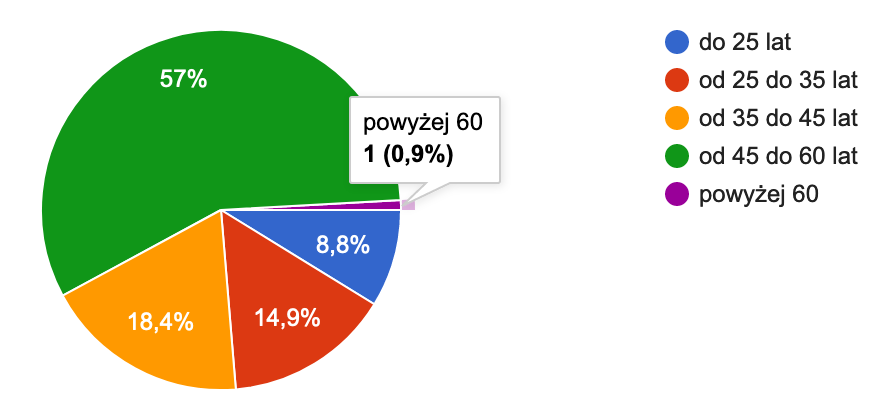
\includegraphics[width=9cm]{char_gr_bad/wiek00}
\caption{Wiek osób ankietowanych. Badania własne 2021/2022 r.}
\label{rys:wiek}
\end{figure}

Opis statystyczny przedstawia tabela \ref{tab:wiek}.

% tabela wiek  - statystyka
\begin {table}[H]
\caption{Statystyki opisowe wieku grupy badanej}
\centering
\begin{tabular}{|l|c|c|}
\hline
Statystyka & Symbol & Wartość\\
\hline
Test Shapiro-Wilk & $p$ & <0,001\\
\hline
liczność danych & $n$ & 115\\
\hline
Średnia & $\bar{x}$ & 44.1\\
\hline
Mediana & $M$ & 52\\
\hline
Odchylenie standardowe & $SD$ & 10.7\\
\hline

\end{tabular}
\label{tab:wiek}
\end{table}



Badaną grupę przedstawioną  na rysunku \ref{rys:plec} stanowi  93,9\%  (108) kobiet i  6,1\%  (7) mężczyzn. Widoczna dysproporcja jest typowa dla rozkładu płci osób zatrudnionych jako pielęgniarki/arze.

% ilustracja płeć
\begin{figure}[H]
\centering
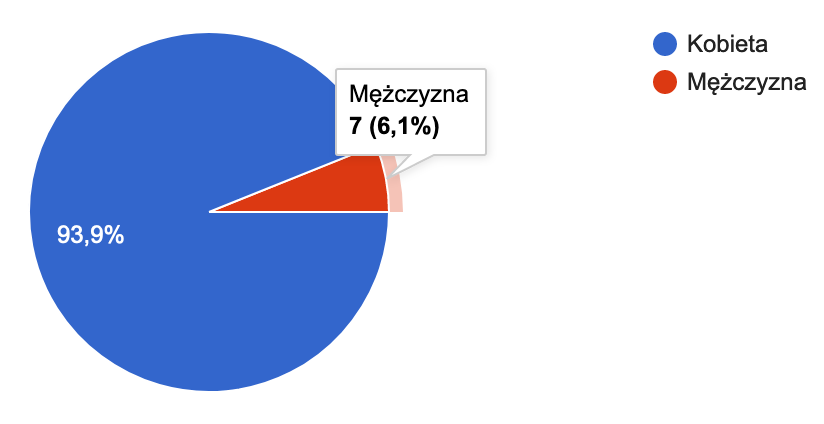
\includegraphics[width=8cm]{char_gr_bad/plec00}
\caption{Płeć osób ankietowanych. Badania własne 2021/2022 r.}
\label{rys:plec}
\end{figure}



Wśród ankietowanych najliczniejszą grupę reprezentowało 57,4\% (66) badanych  z~wykształceniem wyższym - Licencjat Pielęgniarstwa oraz  23,5\%  (27) z tytułem Magistra Pielęgniarstwa. Niektóre osoby zaznaczyły również opcję Liceum Medyczne i  Studium Medyczne. Graficzną reprezentację rozkładu wykształcenia przedstawia rys. \ref{rys:wykszt}. Dodatkowo, rys. \ref{rys:podyplom} ilustruje kształcenie podyplomowe, podejmowane przez badaną grupę. Z pośród 115 respondentów, 20\% (23) miało wykształcenie podyplomowe nie związane z medycyną, 39,1\% (45) ukończyło kurs specjalistyczny, 40\% (46) ukończyło kurs kwalifikacyjny i 
65,2\% (75) ukończyło specjalizację.  


% ilustracja wykształcenie
\begin{figure}[H]
\centering
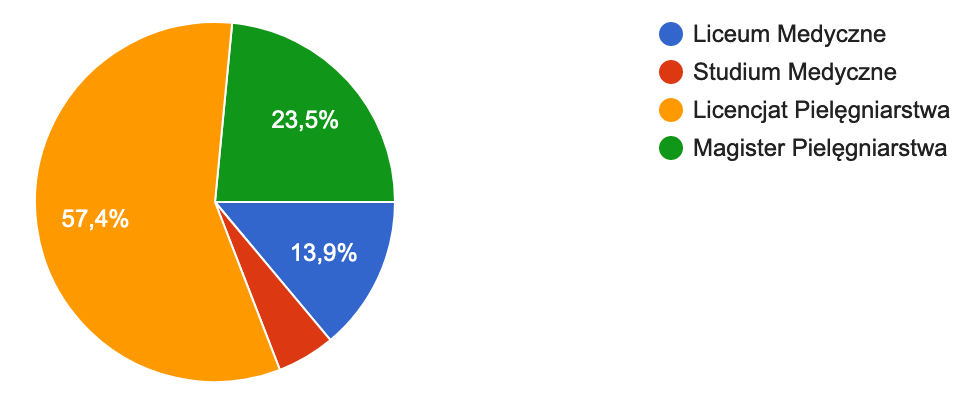
\includegraphics[width=9cm]{char_gr_bad/wyksztalc00}
\caption{Wykształcenie osób ankietowanych. Badania własne 2021/2022 r.}
\label{rys:wykszt}
\end{figure}

\begin{figure}[H]
\centering
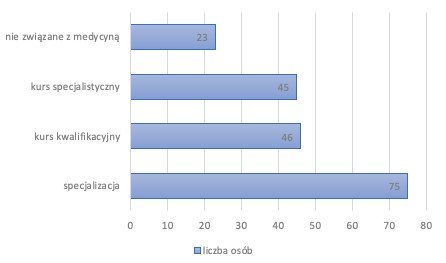
\includegraphics[width=9cm]{char_gr_bad/podyplom01}
\caption{Wykszałcenie podyplomowe osób ankietowanych. Badania własne 2021/2022}
\label{rys:podyplom}
\end{figure}


Zdecydowana większość ankietowanych pozostaje w związku małżeńskim 67,8\%  (78), w związku nieformalnym 17,4\% (20). Pozostałe 15\% to osoby nieżyjące w~związku, w tym  8,7\% (10) rozwiedzione,  5,2\% (6) samotne i 0,9\%  (1) wdowa. Rozkład odpowiedzi ankietowanych pod względem stanu cywilnego ilustruje rys. \ref{rys:cywil}.

% stan cywilny
\begin{figure}[H]
\centering
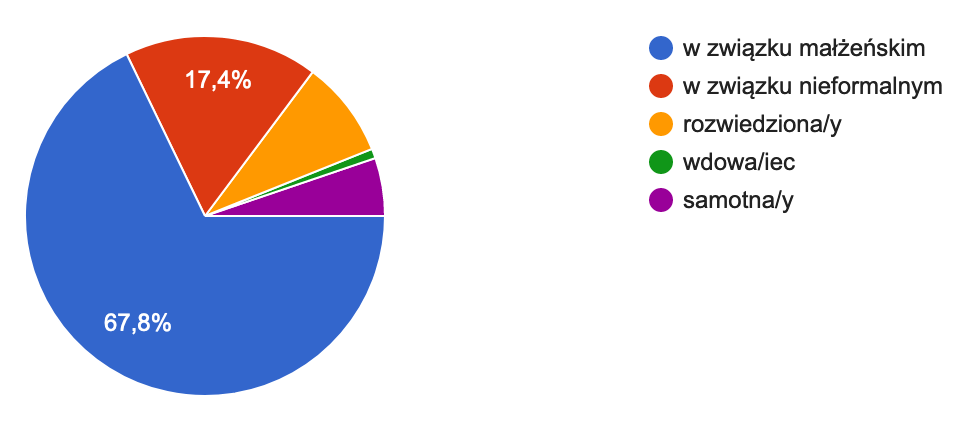
\includegraphics[width=9cm]{char_gr_bad/cyw00}
\caption{Stan cywilny ankietowanych. Badania własne 2021/2022 r.}
\label{rys:cywil}
\end{figure}


Miejsce zamieszkania  respondentów przedstawiono na~rys.~\ref{rys:zamiesz}. Rozkład ten okazał się być dość równomierny. Niewiele powyżej średniej stanowiła grupa 25,2\% (29) zamieszkująca  wsie. Miasta do 50 tys. mieszkańców reprezentowała grupa  20\%  (23). Tak samo liczna grupa zamieszkiwała w miastach od~50 do 150 tys. Nieco mniejsza grupa  18,3\% (21) pochodziła z miast powyżej 150 tys, natomiast z~miast powyżej 500 tys. 16,5\% (19).
% miejsce zamieszkania
\begin{figure}[H]
\centering
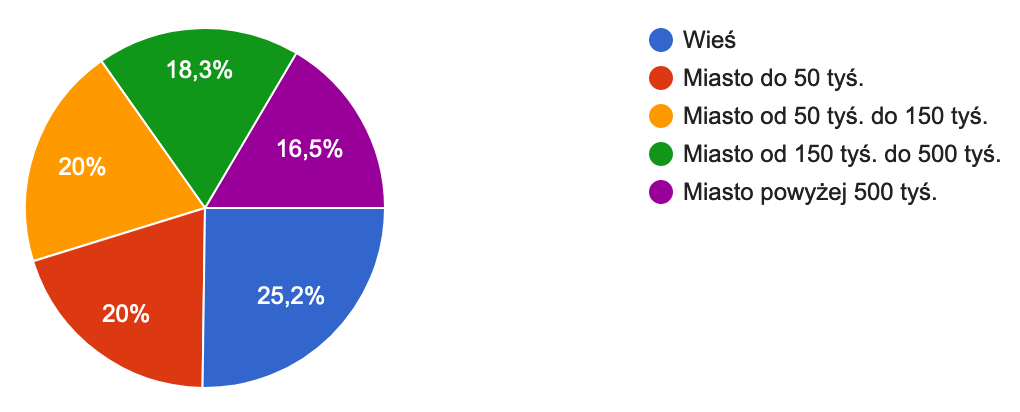
\includegraphics[width=9cm]{char_gr_bad/zamieszka00}
\caption{Miejsce zamieszkania ankietowanych. Badania własne 2021/2022 r.}
\label{rys:zamiesz}
\end{figure}

%-----------------
% Analizy statystyczne
%-----------------
\section{Opis metod analizy statystycznej}

Analizy wykonano w programie GNU PSPP, wer.: 1.4.1, oraz w programie Microsoft Excel, wer 16.60. Konwersję wyników ankiety Google do postaci tabelarycznej wykonano przy pomocy skryptu w języku python wykonanego w programie PyCharm, wer.: 2022.1.1.

\vspace{\baselineskip} 

Wyniki testów statystycznych podano w standardzie APA \cite{apa}:\newline

%\begin{equation}
    \[\chi^2 (lss, n) = x, p=y\]
%\end{equation}

\begin{itemize}
\item[] gdzie:
\begin{description}
\item[$lss$] -liczba stopni swobody
\item[$n$] - liczność zbioru danych
\item[$x$] - obliczona wartość testu $\chi^2$
\item[$y$] - wartość prawdopodobieństwa $p$
\end{description}
\end{itemize}

\vspace{\baselineskip} 

Metody statystyczne, którymi się posłużono, to:
\begin{itemize}
     \item Test Shapiro – Wilka, służy do testowania podobieństwa rozkładu danej zmiennej do rozkładu normalnego. Za pomocą tego testu, sprawdzamy czy interesujące nas zmienne mają rozkłady zbliżone do rozkładu normalnego. Test Shapiro-Wilka testuje hipotezę zerową mówiącą, że rozkład naszej zmiennej jest zbliżony do normalnego. Z tego wynika, że istotny wynik testu Shapiro-Wilka świadczy o tym, że rozkład zmiennej obserwowanej nie jest podobny do rozkładu normalnego \cite{ShapWilk}. 
    
     \item Test Pearsona $\chi^2$, to test nieparametryczny, służący do oceny zależności pomiędzy rozkładem częstości odpowiedzi w zakresie jednej zmiennej, w odniesieniu do drugiej zmiennej.
     
     \item Współczynnik korelacji liniowej Pearsona $R$, określający poziom zależności liniowej między zmiennymi losowymi. Jego wartość może przyjmować wartości od -1 do 1. Na podstawie wartości liczbowej wnioskować możemy o sile związku – im wartość jest bliższa zera, tym siła związku jest słabsza. Wartość dodatnia określa korelację wprost proporcjonalną podczas gdy wartość ujemna okreśa korelację odwrotnie proporcjonalną.
     
     \item Test trendu Mantel-Haenszel $\chi^2$ (Linear-by-Linear association)\cite{mantel}, wykorzystano do oszacowania wspólnego ilorazu szans oraz do sprawdzenia, czy ogólny stopień powiązania jest istotny.
     
%     \item Test Manna – Whinteya opiera się na medianach. Pozwala zweryfikować czy między porównywanymi grupami występują istotne statystyczne różnice. Stosowany jest do porównań pomiędzy dwoma grupami. Stosowany jest w przypadku rozkładów o charakterze różnym od normalnego.
%    
%     \item Test Kruskala – Wallisa test nieparametryczny, opierający się na medianach. Pozwala zweryfikować czy między porównywanymi grupami występują istotne statystyczne różnice. Stosowany jest do porównań pomiędzy więcej niż dwoma grupami. Stosowany jest, gdy w jednej grupie rozkład ma charakter różny od normalnego.
     
\end{itemize}



\chapter*{Wyniki badań}

	Poniżej przedstawiono odpowiedzi respondentów na pytania ankietowe, zał. \ref{app:ankieta}. 
	Wyniki, w postaci tabel, przedstawiono w kolejności użycia w badaniach założonych hipotez i wystąpienia w dyskusji.
	
\vspace{\baselineskip} 

%hip 1

\input wynikitabele/Q32.tex % ZLA  II

\input wynikitabele/Q2.tex  % etaty

\input wynikitabele/Q31.tex

\input wynikitabele/Q3.tex

\input wynikitabele/Q4.tex

\input wynikitabele/Q10.tex

\input wynikitabele/Q11.tex  %traumatyzacja

\input wynikitabele/Q35.tex

\input wynikitabele/Q33.tex

\input wynikitabele/Q13.tex  %uzywki


%hip 2

\input wynikitabele/Q27.tex   % konflikty XII

\input wynikitabele/Q34.tex  % empatia

\input wynikitabele/Q29.tex   % rozpad związku

\input wynikitabele/Q28.tex   % praca powodem niezgody

\input wynikitabele/Q24.tex %uczest w zyciu

\input wynikitabele/Q8.tex

\input wynikitabele/Q18.tex

\input wynikitabele/Q22.tex

\input wynikitabele/Q15.tex   % presja

\input wynikitabele/Q14.tex   % dylemat

\input wynikitabele/Q12.tex   % techniki psychologiczne

%hip 3

	%wspomniane  wyżej

%hip 4

\input wynikitabele/Q20.tex  % satysfakcja z autonomii

\input wynikitabele/Q5.tex   % zadowolona z wyboru drogi zaw.

\input wynikitabele/Q7.tex   % wspierające środowisko

%hip 5

\input wynikitabele/Q21.tex  % wykorzystanie kompetencji

\input wynikitabele/Q9.tex  % systemy motywacyjne

%do dyskusji

\input wynikitabele/Q26.tex  % obowiązki domowe

\input wynikitabele/Q30.tex  % rezygnacja z pracy

\input wynikitabele/Q23.tex  % pasja

\input wynikitabele/Q16.tex  % przemoc

\input wynikitabele/Q19.tex  % strajki

\input wynikitabele/Q36.tex  %perspektywa

\input wynikitabele/Q37.tex  %dziecko



\vspace{\baselineskip} 

%-------------------------
% badania - hipotezy
%-------------------------

\vspace{\baselineskip} 
\large
\textbf{Badania właściwe dla stawianych hipotez}
\normalsize
\vspace{\baselineskip} 

Powyższe wyniki ankiety poddano wstępnej analizie korelacji. Z pomocą programów PSPP oraz Microsoft Excel sporządzono tablicę korelacji przedstawioną w załączniku~\ref{app:tabela}. Tablica ta stanowiła podstawę do dalszej analizy statystycznej.

\vspace{\baselineskip} 
\textbf{Hipoteza 1 - Własne zdrowie, nie jest priorytetem dla pielęgniarek pracujących w ponadnormatywnym czasie pracy.}
\vspace{\baselineskip} 

Test statystyczny wykazał istotną statystycznie różnicę w korzystaniu ze zwolnień lekarskich gdy jest ku temu powód (tab. \ref{tab:Q32}) od ilości etatów,  na których pracuje pielęgniarz/arka (tab. \ref{tab:Q2}). Wartość Mantel-Haenszel $(\chi^2 (1, 115) = 3,87, p=0,049)$. Współczynnik korelacji liniowej Pearsona $(R = -0,2, p=0,049)$. Wartość ujemna tego współczynnika określa tą zależność, jako odwrotnie proporcjonalną: im większa ilość etatów tym rzadsze korzystanie ze zwolnień lekarskich, pomimo iż są do tego wskazania.


Praca mimo choroby (tab. \ref{tab:Q31}), koreluje z ilością godzin pracy (tab. \ref{tab:Q3}) $(R = 0,20, p = 0,038)$, z ~pracą w systemie zmianowym (tab. \ref{tab:Q4}) $(R = 0,26, p = 0,006)$, z "przynoszeniem" do domu emocji z pracy (tab. \ref{tab:Q10}), $(R = 0,33, p < 0,001)$ oraz z odczuwaniem traumatyzacji wtórnej  (tab. \ref{tab:Q11}), $(R = 0,21, p = 0,022)$.

Testy statystyczne wykazały, że osoby doświadczające zjawiska traumatyzacji istotnie  częściej rozpoznają u siebie objawy wypalenia zawodowego ((tab. \ref{tab:Q35})).
Pearson $(\chi^2 (16, 115) = 30,31, p=0,016)$, $(R = 0,29, p = 0,002)$.


Natomiast osoby korzystające ze zwolnień lekarskich, gdy są ku temu wskazania (tab. \ref{tab:Q32}) istotnie  rzadziej doświadczają traumatyzacji (tab. \ref{tab:Q11}), Pearson $(\chi^2 (16, 115) = 40,93, p=0,001)$, $(R = -0,27, p = 0,005)$.


Istotna statystycznie korelacja zachodzi pomiędzy przynoszeniem do domu emocji z pracy (tab. \ref{tab:Q10}), a częstością występowania chorób  (tab. \ref{tab:Q33}), Mantel-Haenszel $(\chi^2 (1, 115) = 6,91, p=0,009)$, $(R = 0,25, p = 0,009)$.

% Q3 vs. Q13
Test statystyczny Pearsona $\chi^2$ wykazał istotne statystycznie różnice, w sięganiu po używki w celu radzenia sobie ze stresem związanym z pracą zawodową  (tab. \ref{tab:Q13}) w ~zależności od ilości godzin pracy miesięcznie (tab. \ref{tab:Q3}) Pearson $(\chi^2 (2, 115) = 6,1152, p=0,047)$. Jednak, co ciekawe, współczynnik korelacji Pearsona $(R = -0,24, p = 0,008)$ ma wartość ujemną co implikuje wniosek, że im więcej godzin pracy, tym rzadziej respondenci sięgają po używki.

%example

%p>0,05

%Test statystyczny nie wykazał istotnych statystycznie różnic poczucia zrozumiałości %(PZR) w zależności od wykształcenia (wartość statystyki testowej Kruskala-Wallisa %5,37; p=0,147).
 
\vspace{\baselineskip} 
\textbf{Hipoteza 2 - Pielęgniarki pracujące w ponadnormatywnym czasie,  mają  trudności w utrzymaniu równowagi w życiu  rodzinnym }
\vspace{\baselineskip} 


%Q27 z Q4 ilosc godzin pracy	%
	Test Pearsona $\chi^2$ wykazał istotną zależność występowania konfliktów na płaszczyznach praca - rodzina (tab. \ref{tab:Q27}), a zmianowym systemem pracy ( tab. \ref{tab:Q4}), Pearson $(\chi^2 (2, 115) = 7,42, p = 0,024)$. Współczynnik korelacji $(R = 0,25, p = 0,008)$ określa, że jest to korelacja wprost proporcjonalna.
	
%Q27 z Q3 ilosc godzin pracy%

	Występuje również  istotna statystycznie zależność nasilenia konfliktów praca - rodzina (tab. \ref{tab:Q27}), od średniej miesięcznej ilości godzin pracy (tab. \ref{tab:Q3}), co oznacza wzrost ilości konfliktów, wraz ze wzrostem godzin pracy.
Mantel-Haenszel $(\chi^2 (1, 115) = 6,37, p=0,012)$, $(R = 0,24, p = 0,011)$.

% mocny	Q27 konflikty z Q34 empatia
	Test statystyczny wskazuje na istotną statystycznie korelację pomiędzy występowaniem konfliktów praca-rodzina (tab. \ref{tab:Q27}), a empatią jako głównym kryterium wyboru zawodu  (tab. \ref{tab:Q34}), Pearson $(\chi^2 (4, 115) = 11,52, p=0,021)$, $(R = 0,26, p = 0,005)$. Co może implikować wniosek, że empatia sprzyja konfliktom na płaszczyźnie praca-rodzina.

% mocny  Q27 z Q28 - pominięty z uwagio na oczywistość relacji	
% mocny  Q27 z Q29	
	Test statystyczny wskazuje na istotną statystycznie korelację prawdopodobieństwa rozpadu związku  (tab. \ref{tab:Q29}), z występowaniem konfliktów praca-rodzina  (tab. \ref{tab:Q27}), Pearson $(\chi^2 (4, 115) = 16,27, p=0,003)$, $(R = 0,29, p = 0,002)$.
	
		%Q28 z Q10
	Istotną statystycznie korelację zaobserwowano pomiędzy przynoszenie "pracy" do domu w postaci myśli i emocji  (tab. \ref{tab:Q10}), a wskazywaniem, że praca zawodowa jest powodem niezgody z partnerem  (tab. \ref{tab:Q28}), Mantel-Haenszel $(\chi^2 (1, 115) = 12,08, p=0,001)$, $(R = 0,33, p = 0,001)$.

Również istotną statystycznie okazała się odwrotnie proporcjonalna zależność uczestnictwa w życiu rodzinnym i przyjaciół, (tab. \ref{tab:Q24}) od ilości etatów, (tab. \ref{tab:Q2}), Mantel-Haenszel $(\chi^2 (1, 115) = 4,02, p=0,045)$, $(R = -0,2, p = 0,045)$. 
	
%1.	1.przynoszenie pracy do domu w postaci myśli i emocji

Zauważono  korelację w postrzeganiu swojego środowiska pracy jako toksyczne (tab. \ref{tab:Q8}), a ilością stresu "przynoszonego" z pracy do domu w postaci myśli i emocji (tab. \ref{tab:Q10}). Test statystyczny Pearsona $\chi^2$ określa tą korelację jako istotną na poziomie $(\chi^2 (16, 115) = 35,4, p = 0,004)$.

Postrzeganie swojego środowiska pracy jako toksycznego (tab. \ref{tab:Q8}), koreluje również z deficytem poczucia bezpieczeństwa w pracy w zagrożeniu koronarowirusem, (tab. \ref{tab:Q18}), Mantel-Haenszel $(\chi^2 (1, 115) = 7,20, p=0,007)$, $(R = -0,3, p = 0,007)$. 

% 2.	Traumatyzacja wtórna Q11
% z Q10 przynoszenie myśli i emocji
Istotną statystycznie korelację wykryto pomiędzy przynoszeniem myśli i emocji z pracy  (tab. \ref{tab:Q10}), a odczuwaniem traumatyzacji wtórnej, (tab. \ref{tab:Q11}), Pearson $(\chi^2 (16, 115) = 76,6, p < 0,001)$.
  
% z Q22 potrzeba psychologa
% z Q35  wypalenie zawodowe
Testy statystyczne wykazały, że respondenci doświadczający zjawiska traumatyzacji wtórnej  istotnie statystycznie częściej odczuwają potrzebę korzystania ze wsparcia psychologicznego  (tab. \ref{tab:Q22}), Pearson $(\chi^2 (16, 115) = 31,37, p = 0,012)$,  $(R = 0,34, p < 0,001)$.

% z Q15 presja społeczna 
% z Q14 dylemat rozwój 
Testy statystyczne wykazały także, że osoby doświadczające zjawiska traumatyzacji wtórnej,  istotnie statystycznie częściej wskazują na problemy związane z presją społeczną wynikającą z oczekiwań wobec Systemu Ochrony Zdrowia (tab. \ref{tab:Q15}), $(R = 0,31, p = 0,001)$, oraz na dylemat wewnętrzny, wynikający z konieczności ciągłego podnoszenia kwalifikacji i wiążącymi się z nim ograniczeniami w życiu osobistym (tab. \ref{tab:Q14}), Pearson $(\chi^2 (16, 115) = 30,69, p = 0,015)$,  $(R = 0,32, p < 0,001)$.


% 3.	Nieumiejętność radzenia sobie ze stresem(techniki)

% Q12 z 10 15 31 32 33 13 	
Badania statystyczne wskazują, że osoby, które lepiej radzą sobie z niwelowaniem stresu  (tab. \ref{tab:Q12}):
	\begin{itemize}
		\item istotnie statystycznie  rzadziej przynoszą "pracę" do domu w postaci myśli i emocji (tab. \ref{tab:Q10}), Pearson $(\chi^2 (16, 115) = 30,49, p = 0,016)$,  $(R = -0,26, p = 0,006)$;
		\item w mniejszym stopniu odczuwają presję społeczną wynikającą z oczekiwań wobec Systemu Ochrony Zdrowia (tab. \ref{tab:Q15}),  Pearson $(\chi^2 (16, 115) = 34,77, p = 0,004)$, $(R = -0,24, p = 0,010)$;
		\item  istotnie statystycznie rzadziej chorują  (tab. \ref{tab:Q33}), Mantel-Haenszel $(\chi^2 (1, 115) = 3,97, p = 0,046)$, $(R = -0,20, p = 0,046)$;
		\item  istotnie statystycznie rzadziej wskazują na wypalenie zawodowe  (tab. \ref{tab:Q35}), Pearson $(\chi^2 (16, 115) = 44,98, p < 0,001)$, $(R = -0,42, p < 0,001)$;
		\item istotnie statystycznie  rzadziej sięgają po używki, w celu niwelowania stresu  (tab. \ref{tab:Q13}), Pearson $(\chi^2 (16, 115) = 31,67, p = 0,011)$, $(R = -0,24, p = 0,009)$.
	\end{itemize}
	

%5.	Dylemat wynikający z podnoszenia kwalifikacji


%6.	Konflikt praca dom i odwrotnie Q27
	% z Q3  Q15  q35 mocny q4 q28 q29 q34   odwrotnie z q7 q24 
	

% słaby	
	%Q27 z Q3 ilosc godzin pracy
	%Q27 z Q35 wypalenie
	%Q27 z Q15 presja społeczna
	
% odwrotny 	Q27 z Q7 pominięto z uwagi na oczywistość
	
%7.	niezgody z powodu pracy w zawodzie
	



% 8.	Wsparcie w godzeniu obowiązków
% Q26 rodzina wspiera  z Q 24 uczestniczy w życiu rodzinnym
% Q26 rodzina wspiera z Q7 wspierające środowisko pracy


%9.	Czynne uczestnictwo w życiu rodzinnym
%  Q24 z  Q23 posiada pasje
%  Q24 uczestniczy w zyciu rodzinnym z -Q35 wypalenie zawodowe
%  Q24 z Q36 uwaza ze dobry wybor
%
%10.	Rezygnacja z zwodu na rzecz szczęścia rodziny
%Q30 rozwaza rezygnacje z Q22 potrzeba psychologa
%Q30 rozwaza rezygnacje z -Q24 nie uczeswtniczy w zyciu rodzinnym
%Q30 rozwaza rezygnacje z Q28 praca powodem niezgody

%11.	Pasja pozazawodowa
%q23 posiada pasje z Q12 potrafi niwelować
%Q12 potrafi niwelować
%
%Q23 posiada pasje to Q12 potrafi niwelowac
%Q23 posiada pasje to Q24 uczestniczy w zyciu rodzinnym
%Q32 posiada pasje to -Q35 nie ma wypalenia


%\vspace{\baselineskip}   

\vspace{\baselineskip} 
\textbf{Hipoteza 3 - Poziom wykształcenia kadry pielęgniarskiej ma istotne znaczenie, dla redukowania skutków traumatyzacji, wynikających z~trudnych sytuacji w pracy.}
\vspace{\baselineskip} 

%1.	Empatia
%2.	Wykształcenie
%3.	Satysfakcja
%4.	Presja wobec systemu
%5.	Dylemat
%6.	Przemoc pacjenta
%7.	Bezpieczeństwo pracy
%8.	Traumatyzacja
%9.	Techniki radzenia

	Test statystyczny wykazał że poziom wykształcenia, rys. \ref{rys:wykszt}, koreluje odwrotnie proporcjonalnie z poczuciem wypalenia zawodowego ( tab. \ref{tab:Q35}), Pearson $(\chi^2 (12, 115) = 29,18, p=0,004)$, $(R = -0,30, p = 0,002)$. Im wyższy poziom wykształcenia, tym niższe poczucie objawów wypalenia zawodowego.
		
	Test statystyczny wykazał że osoby podejmujące więcej kursów podyplomowych i specjalizacyjnych, rys. \ref{rys:podyplom}, mają istotnie statystycznie większe umiejętności niwelowania skutków traumatyzacji  (tab. \ref{tab:Q12}), Mantel-Haenszel $(\chi^2 (1, 115) = 4,82, p=0,028)$. 


	Test statystyczny wykazał że poziom wykształcenia, rys. \ref{rys:wykszt},  istotnie staystycznie koreluje z poczuciem bezpieczeństwa w pracy wobec zagrożenia koronarowirusem  (tab. \ref{tab:Q18}), Mantel-Haenszel $(\chi^2 (1, 115) = 5,72, p=0,017)$, $(R = 0,22, p = 0,017)$. Im wyższy poziom wykształcenia respondentów, tym większe poczucie bezpieczeństwa w~ pracy w zagrożeniu epidemicznym.
	
\vspace{\baselineskip}
\textbf{Hipoteza 4 - Satysfakcja zawodowa pielęgniarek i pielęgniarzy, wynika z~kultury organizacji oraz nabywania kolejnych uprawnień.}
\vspace{\baselineskip}

%1.	Wykształcenie
%2.	Satysfakcja z uprawnien
%3.	Satysfakcja z wyboru drogi zawodowej
%4.	Satysfakcja z perspektywy czasu
%5.	Wspieranie własnego dziecka
%6.	Systemy motywacyjne w pracy


%Q5 zadowolenie z wyboru drogi zawodowej
%  Q7 środowisko  Pana/i pracy, jest wspierające
%  -Q8 toksyczne - pominiete z uwagi na oczywistość
%  -Q11  w mniejszym stopniu odczuwa traumatyzaccje
%  -Q14 mniejszy dylemat
%  -Q15 mniej odczuwa presje
%  -Q35 nie odczuwa wypalenia - pominiete z uwagi na oczywistość

%  Q36 dobry wybor z perspektywy czasu -nie dotyczy
%  Q37 wspierało by dziecko - nie dotyczy
  
  Poziom satysfakcji wynikającej z autonomii zawodu  - nabywania kompetencji, uprawnień, prowadzenia badań naukowych  (tab. \ref{tab:Q20}), istotnie statystycznie koreluje z poziomem wykształcenia, rys. \ref{rys:wykszt}, Mantel-Haenszel $(\chi^2 (1, 115) = 5,94, p = 0,015)$, $(R = 0,23, p = 0,015)$; Im wyższy poziom wykształcenia, tym większe poczucie satysfakcji zawodowej.
  
Wynik testu pokazuje że istnieje istotna korelacja pomiędzy zadowoleniem pracownika z wyboru drogi zawodowej  (\ref{tab:Q5}), a wspierającym środowiskiem pracy, (\ref{tab:Q7}), Mantel-Haenszel $(\chi^2 (11, 115) = 4,50, p=0,034)$, $(R = 0,20, p = 0,034)$.

Testy wykazują istotne statystycznie korelacje większego zadowolenia z wyboru drogi zawodowej  (\ref{tab:Q5}), z:
	\begin{itemize}
		\item rzadziej występującym odczuwaniem dylematu, wynikającego z konieczności podnoszenia kwalifikacji, (tab. \ref{tab:Q14}), Mantel-Haenszel $(\chi^2 (1, 115) = 3,97, p < 0,001)$, $(R = -0,36, p < 0,001)$;
		\item mniejszym odczuwaniem presji społecznej wynikającej z oczekiwań wobec Systemu Ochrony Zdrowia, (tab. \ref{tab:Q15}), Mantel-Haenszel $(\chi^2 (1, 115) = 7,38, p = 0,007)$, $(R = -0,25, p = 0,007)$;
	\end{itemize}

  
  
%Q20 Czy odczuwa Pan/i satysfakcję, wynikającą z autonomii zawodu  - nabywania kompetencji, uprawnień, prowadzenia badań naukowych
% 	z  szkol poziom wykształcenia
% 	Q24 uczestniczy w zyciu rodzinnym


 	
	
%Q36 z perspektywy czasu uważa Pan/i, że dokonał/a dobrego wyboru ścieżki zawodowej? 
%	-Q8 toksyczne - ewidentne

%	-Q10 przynosi emocje
%	-Q14 dylemat rozwój
%	-Q22 potrzeba psychologa
%	Q23 posiada pasje
%	Q24 uczestniczy w życiu rodziny
%	-Q30 rozwaza rezygnacje
%	-Q33 mniej choruje
%	-Q35 nie czuje wypalenia zawodowego

% 	zadna z pozostałych korelacji nie dotyczy hipotezy
   
	

\vspace{\baselineskip} 
\textbf{Hipoteza 5 - Nieadekwatne wykorzystanie kompetencji zawodowych pielęgniarek/rzy  przez SOZ prowadzi do wypalenia zawodowego.}
\vspace{\baselineskip}

%1.	Wspieranie przedstawicieli dla poprawy sytuacji w pielęgniarstwie Q19 - brak korel

%2.	 Wykorzystanie kompetencji Q21 
%		z Q15 presja społeczna
%		z Q35 wypalenie



Test wskazuje  istotny związek między poczuciem niewłaściwego wykorzystania kompetencji pracownika (tab. \ref{tab:Q21}), a odczuwaniem objawów wypalenia zawodowego (tab. \ref{tab:Q35}), Pearson $(\chi^2 (16, 115) = 27,61, p = 0,035)$, $(R = 0,20, p = 0,043)$.

Test statystyczny wykazuje istotną korelacje, dotyczącą braku właściwego wykorzystania kompetencji pracownika  (tab. \ref{tab:Q21}), z presją społeczną wynikającą z oczekiwań wobec Systemu Ochrony Zdrowia (tab. \ref{tab:Q15}), Pearson $(\chi^2 (16, 115) = 47,47, p < 0,001)$, $(R = 0,24, p = 0,012)$.

%, tab. \ref{tab:Q15}, Mantel-Haenszel $(\chi^2 (1, 115) = 7,38, p = 0,007)$, $(R = -0,25, p = 0,007)$;





%4.	Toksyczne środowisko

%
%5.	Q18 odczucie bezpieczeństwa w pracy koreluje 
%	z Q7 wspierajace srodowiso pracy
%	z Q9 systemami motywacyjnymi
%	z -Q15 odwrotnie z presja spoleczna

Poczucie bezpieczeństwa w pracy, tab. \ref{tab:Q18}, istotnie statystycznie koreluje z postrzeganiem środowiska pracy jako wspierającego, tab. \ref{tab:Q7}, Pearson $(\chi^2 (16, 115) = 27,38, p = 0,037)$, $(R = 0,26, p = 0,005)$, oraz z systemami motywacyjnymi, tab. \ref{tab:Q9}, Pearson $(\chi^2 (16, 115) = 23,63, p = 0,023)$, $(R = 0,25, p = 0,008)$
	



\vspace{\baselineskip} 


%-----------------
% Wnioski 
%-----------------
\chapter*{Wnioski}


1. Własne zdrowie, nie jest priorytetem dla pielęgniarek pracujących w~ponadnormatywnym czasie pracy. Im  więcej działalności zawodowej, tym rzadziej  ma miejsce korzystanie ze zwolnienia lekarskiego, mimo, iż są do tego wskazania $( p=0,049)$.

2. Działalność zawodowa w trakcie choroby istotnie statystycznie wpływa na odczuwanie traumatyzacji wtórnej $(p = 0,022)$.

3.  Osoby doświadczające zjawiska traumatyzacji wtórnej,  istotnie statystycznie częściej rozpoznają u siebie objawy wypalenia zawodowego $( p=0,016)$.

4. Występuje  istotna statystycznie zależność między przynoszeniem emocji z pracy, a częstością występowania chorób $(p=0,009)$.

5. Toksyczne środowisko pracy, istotnie statystycznie wiąże się z przynoszeniem stresu do domu w postaci myśli i emocji $( p = 0,004)$.

6. Osoby doświadczające traumatyzacji wtórnej istotnie statystycznie wyrażają potrzebę wsparcia psychologicznego $(p = 0,012)$.

7. Osoby doświadczające traumatyzacji wtórnej podlegają presji społecznej  wynikającej z oczekiwań wobec SOZ $(p = 0,001)$ oraz odczuwają dylemat wewnętrzny wynikający z konieczności podnoszenia kwalifikacji $ (p = 0,015)$.

8. Osoby pracujące w ponadnormatywnym czasie wykazują konflikt na płaszczyźnie praca/rodzina. Im więcej godzin pracy, tym więcej konfliktów $( p=0,012)$.  Wykazano również, konflikty ze względu na pracę zmianową $(p = 0,024)$.

9. Zaobserwowano istotny statystycznie związek między przynoszeniem do domu myśli i emocji z pracy, a wskazywaniem, iż praca jest powodem niezgody z partnerem $(p = 0,001)$.

10. Wykazano istotny statystycznie związek między podnoszeniem kwalifikacji zawodowych, a umiejętnością niwelowania skutków traumatyzacji $(p=0,028)$.

11. Wykazano istotny statystycznie związek między poziomem wykształcenia, a~wypaleniem zawodowym. Im więcej aktywności edukacyjnej, tym mniejsze ryzyko wypalenia zawodowego $(p=0,004)$.


12. Poziom satysfakcji wynikającej z autonomii zawodu istotnie statystycznie koreluje z poziomem wykształcenia. Im wyższy poziom wykształcenia, większa liczba ukończonych kursów, specjalizacji, tym większa satysfakcja $(p = 0,015)$.

13. Nieadekwatne wykorzystanie kompetencji zawodowych przez SOZ stanowi ryzyko wypalenia zawodowego $ (p = 0,035)$.

14.  Systemy motywacyjne i  wspierające środowisko pracy, sprzyjają poczuciu bezpieczeństwa w miejscu aktywności zawodowej $(p = 0,023)$.



\vspace{\baselineskip} 
\large
\textbf{Rekomendacje i kierunki kolejnych badań.}
\normalsize
\vspace{\baselineskip} 



Prezentowane badania mają kilka ograniczeń. W związku z tym, że ankieta była przeprowadzana on-line, nie można mieć pewności, że, odpowiedzi udzielali tylko i wyłącznie studenci WSM w Legnicy. Również osobisty charakter pytań, może powodować tendencyjność odpowiedzi. Odpowiedzi na pytania mogą się różnić w~zależności od własnych doświadczeń,  czy obecnej sytuacji zawodowej i osobistej. Mimo tych ograniczeń, należy uznać, iż wyniki badania są reprezentatywne i wnoszą istotne informacje na temat wpływu pracy zawodowej na życie osobiste pielęgniarek i~pielęgniarzy.


Niniejsza praca badawcza, zwraca uwagę, na niepokojące zjawiska tj. pracę w~ponadnormatywnym czasie, niekorzystanie ze zwolnień lekarskich, gdy są do tego wskazania i wykonywanie działalności zawodowej w tym czasie, stosowanie używek, czy brak poczucia bezpieczeństwa w pracy zawodowej.

1.	 Uzyskane wyniki ewidentnie wskazują, iż pielęgniarki są obarczone pracą w ponadnormatywnym czasie. Aby zapobiegać obniżonej jakości pracy, należy wprowadzić skuteczne rozwiązania systemowe, sankcjonujące pracę w nadgodzinach. Zarządzający placówkami ochrony zdrowia powinni zmierzać do wprowadzenia odpowiednich procedur, które zapewnią bezpieczeństwo pracy personelowi i~bezpieczeństwo pacjenta.

2.	Zarządzający zasobami ludzkimi w zakładach opieki medycznej, powinni zapewnić szkolenia i możliwości rozwoju zawodowego w zakresie treningu empatii, komunikacji, technik psychologicznych walki ze stresem. Powinni kształtować wspierające środowisko pracy, reagując na informacje zwrotne płynące od personelu i chronić go przed traumą. Działania te muszą być zgodne z harmonogramem pracy pracownika. W sytuacji niezwykle traumatycznej dla pracownika, zespołu powinno się udzielić krótkiego urlopu, a jeśli nie jest to możliwe, zapewnić przesunięcie do pracy, która wymaga zaangażowania na innym polu.

3.	Powinno się dążyć do pozytywnego wzmacniania personelu, stosowania systemów motywacyjnych, regularnego wspierania przez afirmację sukcesu: terapeutycznego, zawodowego i osobistego.

4.	Powinno się promować pielęgniarstwo jako prestiżowy zawód, zarówno lokalnie jak i globalnie w mediach, poprzez wywiady, akcje informacyjne z osobami z osiągnięciami w dziedzinie pielęgniarstwa, Powinno się podkreślać znaczenie EBM.

5.	Powinno się dążyć, do maksymalnego wykorzystania uprawnień i kompetencji zawodowych pielęgniarek, by podnieść rangę zawodu. Należy, również skorzystać z~doświadczenia zawodowego pielęgniarek z wieloletnim stażem, o wysokim poziomie satysfakcji zawodowej, a niskim poziomie wypalenia zawodowego, gdyż są cennym źródłem wiedzy o funkcjonowaniu w środowisku pracy.

6. Powinno się kształtować następne pokolenia zawodów medycznych do  wspólnego działania w zespołach terapeutycznych, opartych na partnerstwie i wzajemnym szacunku dla innego zawodu, co przekłada się na profesjonalizm, efektywność, jakość opieki wyrażonej zadowoleniem pacjentów i obniżonymi kosztami poniesionymi przez pracodawców.


Implikacje te wskazują na interesujące kierunki przyszłych dociekań naukowych.


%-----------------
% Dyskusja
%-----------------
\section*{Dyskusja}
\textit{Dyskusja jest częścią krytyki metodologicznej i stanowi swoistą metametodę, leżącą u podstaw współczesnego myślenia naukowego, jak i stały element metod, w ramach których można ją sensownie realizować} \cite{krytyka}.


Celem badania własnego było określenie wpływu pracy zawodowej na życie osobiste pielęgniarek i pielęgniarzy czynnych zawodowo. To zagadnienie było obiektem zainteresowań badaczy różnych specjalności. Zarówno socjologów, psychologów jak i zarządzania w systemie ochrony zdrowia.  Dzięki temu, możliwe jest szerokie spojrzenie na życie, specyficznej grupy zawodowej jaką są pielęgniarki. Możliwe jest zaobserwowanie pewnych zjawisk, np. wypalenia zawodowego, określenie przyczyn ich występowania, a następnie wdrożenie działań profilaktycznych, naprawczych czy protekcyjnych. Wyniki kolejnych badań wzbogacają wiedzę, służą rozwojowi pielęgniarstwa. Ze względu, iż temat jest rozległy i obejmuje wiele dziedzin życia społecznego, badacze nadal poszukują odpowiedzi na pytania : czy wykonując tak odpowiedzialny i wyczerpujący zawód, można prowadzić szczęśliwe życie osobiste? Czy empatia pomaga, czy przeszkadza w~wykonywaniu tego zawodu? Jakie niebezpieczeństwa dla własnego zdrowia niesie działalność zawodowa w~ponadnormatywnym wymiarze czasu pracy? Niniejsza praca również podejmuje próbę odpowiedzi na te pytania.

Poziom świadomości pielęgniarek i pielęgniarzy na temat zagrożeń, wynikających z pracy w ponadnormatywnym czasie pracy, powinien mieć istotne znaczenie na decyzję o podjęciu dodatkowej działalności zawodowej. Przeważająca liczba badaczy skłania się do wniosków, iż praca w ponadwymiarowym czasie pracy jest szkodliwa i obciążająca dla organizmu człowieka. Jednocześnie istnieją badania, w których podkreśla się, iż,  regularne, rotujące się systemy zmianowe: jeden do trzech dni na tej samej zmianie roboczej, uważa się za biologiczne i społecznie mniej obciążające, niż systemy tygodniowe \cite{konflikt}. Świadomość tego faktu  jest niewystarczająca, lub schodzi na plan dalszy, wobec różnych potrzeb, które podlegają zmianom w trakcie życia.



  W pracy poglądowej \textit{ Wymiar czasu pracy kontra zdrowie - przegląd doniesień naukowych} autorki Zużewicz i  Pędrecka przekonują że pracownicy będący w stanie wielogodzinnej aktywności, nie są w stanie wykonywać powierzonych im zadań odpowiedzialnie i efektywnie, co zwiększa ryzyko zagrożenia zdrowia pacjenta jak i samych sprawujących opiekę \cite{kontra}. 

W czerwcu 2021 r Stowarzyszenie Pielęgniarki Cyfrowe przeprowadziło badanie sondażowe, w którym wzięło udział 2459 osób. Przeważająca większość (91,9\%)  to pielęgniarki i pielęgniarze,  położne/i   stanowili 8,1\% tej grupy badanych.  Prawie wszyscy ankietowani (94,3\%  ) w podstawowym miejscu pracy  są zatrudnieni  w pełnym wymiarze etatu. Pozostali wykonują zawód na podstawie innych form zatrudnienia.  Dodatkowo 45,4\%  respondentów  jest zatrudnionych w formie: kontraktów, umów zlecenia, a nawet cały etatu.  Osoby zatrudnione w ramach umowy o pracę deklarowały powyżej 200 godzin pracy w miesiącu.  Zdecydowana większość respondentów podawała iż powodem dodatkowej pracy są względy ekonomiczne, plany życiowe - 25,7\%,  podstawowa egzystencja -  23,1\%.  Na dodatkowe dyżury z powodu braków kadrowych godzi się  9,5\% sondowanych.  Pojawiły się również powody: samotność, pracoholizm, chęć samorealizacji \cite{cyfrowe}. Wykładnia prawa, wyraźnie mówi, że zasadnicze normy czasu pracy obowiązujące pracowników podmiotów leczniczych wynoszą na dobę 7 godzin i 35 minut na dobę, oraz 37 godzin i~55 minut na tydzień. Jest to średnia, której nie można przekraczać w trzymiesięcznym okresie rozliczeniowym \cite{okres}. Ustawa o działalności leczniczej nie reguluje  jednak wprost limitu pracy w godzinach nadliczbowych. Pośrednio wynika to z maksymalnej normy czasu pracy w wymiarze 48 godzin tygodniowo \cite{klauzula}. Natomiast prawie połowa  ankietowanych badania własnego  spędza w pracy od 170 do 260 godzin.  Przekłada się  to np. przy 170 godzinach na około:  7~dyżurów dobowych, 14 dyżurów dwunastogodzinnych. Przy 260 godzinach te liczby to: około  10 dyżurów dobowych,  20 dyżurów dwunastogodzinnych. W badaniach własnych, w których wzięło udział 115 studentów i absolwentów Wyższej Szkoły Medycznej  w Legnicy na kierunku pielęgniarstwo drugiego stopnia, znaczna część respondentów pracuje w jednym miejscu pracy, około 30\% w dwóch, a tylko 7\% w więcej niż dwóch.  Ze 115 respondentów  14 badanych  pracuje powyżej 200 godzin miesięcznie, co stanowi, 12,2\% ankietowanych,   ośmiu respondentów deklaruje pracę powyżej  240 godzin miesięcznie, jednak rekordzistki w trakcie indywidualnych rozmów przyznają się do 72 godzin nieprzerwanej pracy, 470 godzin miesięczne, bądź 2 dni wolnych od pracy zawodowej w miesiącu.  



Wykonywanie obowiązków zawodowych w trakcie aktywnej choroby własnej, czy bliskiego, świadczy o prawdziwości założonej hipotezy $( p=0,049)$. Jest to wysoce niepokojące zjawisko, gdyż aby wykonywać swoje zadania w pracy zawodowej, pracownicy muszą stosować   leki, które  zniwelują objawy choroby. Abstrahując od etycznego wymiaru takich działań,  ich konsekwencji dla pacjenta, placówki, to niosą one konkretne skutki dla zdrowia pielęgniarki. Metha i współpracownicy opublikowali w marcu 2022 wyniki ogólnokrajowego prospektywnego, kohortowego badania  w~USA. Czternaście tysięcy pięćset czterdzieści dwie  pielęgniarki w wieku 25-42 lata uczestniczyło w badaniu Nurses Health Study II. W przedziale czasowym 1989/2018,  co dwa lata monitorowano stosowanie przez nie antybiotyków i ~jednocześnie przeprowadzano testy poznawcze. Wyniki porównywano z danymi osób, które przyjmowały antybiotyków niewiele lub nie przyjmowały ich wcale. Wyniki były niepodważalne: pielęgniarki, które często, czy długotrwale stosowały antybiotyki uzyskały zdecydowanie niższe parametry uczenia się, pamięci roboczej, szybkości motorycznej czy utrzymania uwagi. Sytuację taką autorzy tłumaczą przyśpieszonym starzeniem mózgu, nawet o 3-4 lata.  Co dla  pielęgniarki polskiej o~średniej wieku - 53 lata, powinno mieć znaczenie \cite{statystyka}.  Naukowcy  wiążą zaburzenia poznawcze z  kondycją mikrobiomu jelitowego \cite{metha}. Natomiast Trinkoff i współautorzy donieśli w 2011 roku, że w szpitalach o wyższym wskaźniku umieralności, pracuje większy procent pielęgniarek, które nie korzystają z przerw w pracy, nie biorą urlopów, i pracują chore \cite{trinkoff}.


Nie bez znaczenia jest fakt, że zagrożenia  dla zdrowia, wynikające z pracy w~ponadnormatywnym wymiarze mogą ulec intensyfikacji czy zniwelowaniu, poprzez kulturę organizacji. Na uwagę zasługują wnioski z badania \textit{mobbing w środowisku pracy pielęgniarek} przeprowadzonego za pomocą sondażu diagnostycznego wśród pielęgniarek województwa świętokrzyskiego w 2010 roku. Gdzie zaobserwowano działania dyskryminacyjne i o charakterze mobbingowym wobec personelu podnoszącego swoje kwalifikacje i wykształcenie. W badaniu tym dokonano porównań z podobnymi w~województwie śląskim, mazowieckim i zachodniopomorskim \cite{mobbing}. Z kolei Żuchowski w badaniach, przeprowadzonych na terenie województwa mazowieckiego i podlaskiego, w którym wzięło udział 140 respondentów, wykazuje, że zjawisko mobbingu kadry zarządzającej pielęgniarkami, w stosunku do podwładnych to liczba, rzędu 27,8\% \cite{zuchowski}. Z danych Ogólnopolskiego Klubu Antymobbingowgo wynika, iż liczba pracowników Ochrony Zdrowia jest niedoszacowana i na pewno wyższa, mimo,  iż termin mobbing wprowadzono do znowelizowanego Kodeksu Pracy w 2004 roku \cite{grabowski}, \cite{kodeks}. Analiza wyników badania własnego pokazuje, iż 34,8\% (40) ankietowanych uważa, że środowisko miejsca pracy jest toksyczne,  oraz że występuje mobbing i hejt.


Wypalenie zawodowe jest ogromnym problemem pracowników ochrony zdrowia. Jednocześnie, ta grupa zawodowa jest na nie najbardziej narażona z pośród pracowników innych profesji \cite{wypal}. Rezmerska i współautorki, w badaniach na temat \textit{specyfiki pracy, a wypalenia zawodowego w opinii pielęgniarek},  przekonują, iż poziom wypalenia zawodowego, jest zróżnicowany w zależności od specyfiki oddziału. Jest on wyższy, w oddziałach zabiegowych i  u pielęgniarek pracujących w systemie zmianowym \cite{zmiany}. Natomiast Breisert w badaniach przeprowadzonych w Poznaniu na grupie 138 pielęgniarek pokazuje, że najwięcej osób wypalonych zawodowo jest zatrudnionych na pediatrii, onkologii i psychiatrii, natomiast zadecydowanie mniej na internie. Wymagania dotyczące specyficznego kontaktu z chorym dzieckiem, czy pacjentem z~chorobą nowotworową,  a także nieustanne stykanie się z cierpieniem,  przewlekły stres oraz brak poczucia sensu własnej działalności, obciążenie pracą, brak systemów motywacyjnych, niewspółmierne zarobki składają się na stały wzrost  pielęgniarek/rzy wypalonych zawodowo \cite{breisert}. Zjawisko wypalenia zawodowego nie jest obce uczestnikom analizy własnej.

  
 
 
  Znaczna część uczestników badania,  twierdzi, że przynosi pracę do domu w~postaci myśli i emocji. Respondenci, którzy doświadczają traumatyzacji wtórnej stanowią prawie czterdzieści procent badanej społeczności. W badanej grupie blisko czterdzieści procent potrafi niwelować objawy takie jak: smutek, żal, poczucie bezradności, przewlekły stres, niewiele mniej osób  przyznaje, że nie potrafi stosować technik psychologicznych do poradzenia sobie z sytuacją trudną.  Aby rozładować stres niektórzy  sięgają  po używki.   Dodatkowo prawie połowa opiniodawców odczuwa dylemat wewnętrzny, wynikający z konieczności ciągłego podnoszenia kwalifikacji, co wiąże się z ograniczeniami w życiu osobistym.  Przy tak kategorycznych danych 80\% badanych  stwierdza, że w ich życiu nie występuje konflikt na linii praca/rodzina i~odwrotnie, a  73 \%  z nich uważa, że praca nie jest powodem niezgody z~życiowym partnerem.  Także 77,4\%   sondowanych  twierdzi, że są wspierane w godzeniu obowiązków domowych z pracą, tyle samo ankietowanych ma czas dla rodziny i~czynnie uczestniczy w życiu rodzinnym i imprezach okolicznościowych. Tylko 16,5\%  kiedykolwiek rozważało rezygnację z zawodu, na rzecz szczęścia rodziny. Równie spektakularnym wynikiem jest odpowiedź na pytanie o pasję pozazawodową, aż 72,2\%  podało, iż rozwija pasję pozazawodową. Dane te potwierdzają hipotezę, o trudnościach w utrzymaniu równowagi  w życiu rodzinnym, przez osoby wykonujące pracę w ponadnormatywnym wymiarze  $(p=0,012)$.  Z kolei  Nowak-Starz i pozostali autorzy przeprowadzili badania na temat \textit{ wpływu stresu związanego z pracą zawodową na występowanie wypalenia zawodowego u pielęgniarek pracujących w oddziałach zabiegowych i zachowawczych}. Wykazali oni, że wśród 103 uczestników badania 90\% stwierdziło, że  praca zawodowa ujemnie wpływa na ich życie rodzinne. Wskazali oni  własne objawy wypalenia zawodowego, a pielęgniarki, które przynosiły negatywne emocje z pracy do domu, charakteryzowały się brakiem satysfakcji zawodowej. \cite{nowak}. W badaniach  przeprowadzonych w Centrum Onkologii w Bydgoszczy, w 2011 roku, na grupie 72 pielęgniarek i pielęgniarzy, dotyczące analizy jakości życia pracowników ochrony zdrowia, Kurowska i Klatt  wykazują, że w badanej grupie wystąpił wysoki poziom wsparcia ze strony partnera życiowego. Także ogólne wsparcie rodziny, było na poziomie wysokim, przy czym najwyżej oceniono wsparcie emocjonalne \cite{poziom}. Natomiast w 2017 roku zespół badaczy Polskiego Pomiaru Postaw i Wartości przeprowadził badanie, w którym wzięło udział 1627 osób z zawodowej grupy pielęgniarskiej. Zdecydowanie większa liczba osób deklarowała, że udaje się jej zachować równowagę między działalnością zawodową i rodzinną - 30,6\% było zdecydowanych w tej kwestii, a 42,1\% podało odpowiedź, że taką równowagę raczej zachowuje. Tylko 28\% badanych osób, byłoby skłonnych zrezygnować z pracy, dla dobra rodziny. W tym badaniu  56,7\% neguje wpływ pracy na życie rodzinne i twierdzi, że potrafi zachować dystans między pracą, a czasem z rodziną, ale 37\% nie posiada takiej umiejętności. \cite{komunikat}.
Podsumowując dyskusję na ten temat, należy wyrazić uznanie dla osób wybierający zawód wymagający ciągłego doskonalenia i niosący ogrom poświęceń w życiu osobistym, jednocześnie realizując obie role.

Zawodowa grupa pielęgniarska, kształci się, aby niwelować skutki traumatyzacji, wynikające z trudnych sytuacji w pracy $(p=0,028)$. Traumatyzacja wtórna określana do niedawna jako zmęczenie współczuciem, przypisywanym pielęgniarkom, a następnie innym zawodom pomocowym, spowodowała przeniesienie traumy z osoby cierpiącej  na terapeutę \cite{figley}. Na traumatyzacje narażone są osoby o wysokim stopniu inteligencji emocjonalnej. Zwłaszcza jej składowej empatii. Natomiast Wilczek-Rużyczka twierdzi na podstawie wieloletnich badań własnych i analizy wyników badań innych badaczy, że empatia pełni rolę ochronną, a \textit{wysoki poziom empatii, jest nie tylko wartością psychologiczną, terapeutyczną, lecz również powinnością moralną i staje się kryterium profesjonalizmu.  Pielęgniarka wchodząc w relację z pacjentem, odczuwa bliskość, która zaspokaja często potrzeby obu stron, jednocześnie nie traci własnej tożsamości} \cite{wilczek}.  Interesujące wnioski płyną z badania przeprowadzonego na Uniwersytecie w~Pekinie. Naukowcy przydzielili pacjentów oddziału onkologicznego trzem grupom pielęgniarek/rzy. 365 pacjentów z nowotworami płuc, wspierały pielęgniarki o wysokim, średnim i niskim poczuciu empatii,  w okresie od października 2016 do maja 2017.  Pacjenci, którym towarzyszyły pielęgniarki o wysokim poziomie empatii, mieli większy procent limfocytów B i komórek NK w momencie wypisu \cite{nk}. W badaniu własnym część respondentów, podała właśnie empatię, jako główne kryterium wyboru zawodu. Trening empatii oraz kształcenie się w  rozpoznawaniu, niwelowaniu niekorzystnych skutków traumatyzacji,  ma ogromne znaczenie dla życia osobistego pielęgniarki. Biorący udział w badaniu własnym,  posiadają wykształcenie wyższe,  znamienita większość zdała egzamin specjalizacyjny. Ankietowani wykazują posiadanie uprawnień zawodowych potwierdzonych zaświadczeniami, certyfikatami i~dyplomami, również niezwiązanymi z zawodem wykonywanym, także magistra innego kierunku. Wśród wielu czynników ryzyka wtórnej traumatyzacji wymienia się poziom wykształcenia. Wyższe wykształcenie oraz poczucie satysfakcji z pracy pełni rolę ochronną, natomiast osoby o niższym stopniu wykształcenia są bardziej podatne, na zmęczenie współczuciem \cite{oginska}.


W przytoczonym wcześniej komunikacie z badań na temat życia rodzinnego i zawodowego, znaczna część opiniodawców uznała, że zawód wymaga od nich nieustannego podnoszenia kwalifikacji zawodowych \cite{komunikat}. Natomiast prawie  pięćdziesiąt  procent respondentów  badania własnego  odczuwa dylemat wewnętrzny, związany z~ koniecznością ciągłego podnoszenia kwalifikacji.
 Blisko trzydzieści procent  badanych analizy własnej  zdecydowanie czuje presję społeczną, wynikająca z oczekiwań wobec systemu ochrony zdrowia,  ponad trzydzieści procent   przychyla się do tego wariantu odpowiedzi.  W badaniu własnym 46\%  ankietowanych doświadczyło przemocy słownej lub fizycznej ze strony pacjenta, a 33\%  przyznało, że  raczej jej doświadczyło.  Grudzień i współpracownicy w pracy oryginalnej - \textit{opinie personelu medycznego na temat agresywnych zachowań pacjentów} przedstawiają wyniki badania sondażowego, w którym udział wzięło 115 przedstawicieli zawodów medycznych. Wyniki są zbliżone do badania własnego - 46,2\% to kontakt z agresją w~stosunku do pielęgniarek. Jest to zarówno agresja słowna, wulgaryzmy oraz lekceważące wypowiadanie się o personelu \cite{grudzien}. 

  Prawie połowa ankietowanych nie  czuje się bezpiecznie w pracy w zagrożeniu koronarowirusem. Jest to niepokojący wynik, biorąc pod uwagę, że pandemia została znacznie ograniczona przez szczepienia antywirusowe, choć  jest to liczba zdecydowanie mniejsza, niż na początku epidemii, gdzie fundamentalne prawo pracownika, do bezpieczeństwa własnego w pracy i poza nią, utraciło moc.


 Ogińska-Bulik w badaniach przeprowadzonych w 2019 roku na grupie 200 przedstawicieli personelu medycznego, w tym 35\% stanowiły pielęgniarki, przedstawia wyniki wskazujące na wysokie i średnie nasilenie wtórnego stresu wśród pracowników po traumie. Wnioski zachęcają do \textit{rozwoju umiejętności i korzystania ze wsparcia społecznego, w celu redukowania negatywnych i występowania pozytywnych konsekwencji wtórnej ekspozycji na traumę} \cite{trauma}. 
  Umiejętności takie posiada prawie 40\% badanych studentów WSM,  a  50\% z nich zgłasza potrzebę korzystania ze wsparcia psychologicznego dla pracowników medycznych.

Satysfakcja zawodowa pielęgniarek i pielęgniarzy, wynika z kultury organizacji oraz nabywania kolejnych uprawnień $(p=0,015)$. Hipotezę tę poddano weryfikacji osób badanych.  Blisko 60\%  z nich,  odczuwa satysfakcję, wynikającą z autonomii zawodu: nabywania kompetencji, uprawnień, prowadzenia badań naukowych.  Nawet  85,2\%   uczestników badania własnego jest zadowolona z wyboru drogi zawodowej. W badaniach Borowskiej i współpracowników  wśród 130 aktywnych zawodowo pielęgniarek  Uniwersyteckiego Szpitala Klinicznego w Białymstoku, 41,5\% osób określiło własną satysfakcję zawodową jako wysoką, a 63\% czuło się docenioną w~pracy zawodowej. Zdaniem co trzeciej osoby, atmosfera w pracy ma kluczowe znaczenie dla poczucia satysfakcji zawodowej. Pielęgniarki - 60\% respondentów w~tym badaniu określiło  pozycję swojego zawodu, wśród innych zawodów na poziomie średnim. W pytaniu o prestiż zawodu, ankietowani - 45\% uznali kwalifikacje zawodowe, 40\% wykształcenie, 33\% samodzielność i niezależność zawodu \cite{zbiorowa}. Interesujące są również badania Skorupskiej  i Machowicz, gdzie badani w 92\% uważają, że pielęgniarka jest równorzędnym członkiem zespołu w opiece nad pacjentem \cite{skorupska}. O ocenę poziomu satysfakcji zawodowej wśród pielęgniarek onkologicznych pokusiły się również  organizatorki 22 ogólnopolskiej konferencji pielęgniarek onkologicznych w Białymstoku w 2018 roku. Badaniu poddało się dobrowolnie 218 uczestniczek z ośrodków onkologicznych w kraju. Średnia wartość satysfakcji z pracy wyniosła 67,10 punktów. Uczestniczki podkreślały zadowolenie z umiejętności zawodowych swojego przełożonego i wagi własnej pracy. Co ciekawe nie wykazano zależności satysfakcji z~wykształceniem, ani stażem pracy. Natomiast wyższy poziom satysfakcji prezentowały osoby w związkach małżeńskich \cite{onkologiczne}. Znaczna część respondentów  badania własnego uważa z perspektywy czasu, że dokonało właściwego wyboru ścieżki zawodowej, a 56,5\%  ankietowanych wspierałoby własne dziecko, gdyby chciało się spełniać w~pielęgniarstwie. Wyniki badań   YouGov Survey into Professional Perception,  wskazują iż  jeden na trzech polskich rodziców (33\%) byłby niezadowolony z wyboru pielęgniarstwa jako drogi zawodowej, przez własne dziecko.  Jest to, najniższy odsetek negatywnych odpowiedz spośród 16 krajów biorących udział w badaniu. Tylko czterech na dziesięciu rodziców (38\%) wsparłoby własne dziecko w tej drodze, zarówno duchowo jak i materialnie. To  z kolei najniższy wynik odnotowany w Europie. Na świecie, niżej od Polski plasuje się  Meksyk (37\%) i Chiny (30\%). Badanie to było przeprowadzone wśród  22000 uczestników. Dane te  w odniesieniu nie tylko do kraju, mogą wskazywać, że pielęgniarstwo, staje się coraz mniej popularnym zawodem \cite{yougov}.

Satysfakcja zawodowa, to również systemy motywacyjne, jednak 36,5\% respondentów podkreśla, że w zakładzie pracy, w którym pracuje, zdecydowanie nie stosuje się systemów motywacyjnych. Tylko 13,9\% twierdzi, że raczej istnieją takie systemy, natomiast nikt z uczestników badania, nie zaznaczył wariantu, o~zdecydowanym występowaniu systemów motywacyjnych.  Niewielu  ankietowanych uważa, że środowisko pracy jest zdecydowanie wspierające, a 48,7\%  sądzi  iż jest raczej wspierające. Natomiast zdecydowanie toksyczne środowisko pracy występuje u 7\%  ankietowanych, a 27,8\%  podało odpowiedź \textit{raczej tak}, w pytaniu dotyczącego toksycznego środowiska pracy.  Przekrojowy sondaż Aiken i współpracowników wśród  33 tysięcy 659 pielęgniarek w 488 szpitalach w 12 krajach europejskich wykazał niezadowolenie z pracy  od 11 do 56\% badanych, 19 do 49\% planowała odejść z~ pracy \cite{termedia}. Podobne wnioski płyną z~wyników badań Dallora i współpracowników, gdzie 26\% pielęgniarek i pielęgniarzy jest bardzo, albo raczej nieusatysfakcjonowanych pracą zawodową \cite{dalora}. Na toksyczne środowisko pracy, składa się wiele elementów. Między innymi relacje interpersonalne w grupie zawodowej, a także w zespole terapeutycznym. Szczególnie jest to widoczne w relacjach pielęgniarka/lekarz, gdzie mimo samodzielności zawodu pielęgniarskiego, często jest on postrzegany przez lekarzy jako zawód wykonawczy im  podległy, co sprzyja konfliktom i niezdrowej atmosferze w pracy. Zauważa się potrzebę zmian w myśleniu o pielęgniarce jako partnerze w~procesie leczenia. Świadczą o tym projekty obozów wakacyjnych dla studentów rożnych kierunków medycznych, by mogli się poznać, wspólnie wykonać zadania i~zrozumieć, że razem są silniejsi, sprawniejsi i bardziej skuteczni. Projekt ten trwa od ponad 35 lat i został zapoczątkowany przez profesora Jacka Imielę propagatora idei współpracy międzyzawodowej \cite{imiela}.

Wiedzę i postawy pielęgniarek na temat praktyki opartej na dowodach naukowych oceniała Gotlib i współautorzy Warszawskiego Uniwersytetu Medycznego w 2014 roku. Uczestnicy badania znali znaczenie terminu EBM w 42\%, dla 34\% to nowoczesne wykonywanie zawodu, 36\% zamierza aktualizować wiedzę zgodnie z~doniesieniami naukowymi, a 41\% uważa, że są one przydatne w praktyce zawodowej \cite{gotlib}.  Również Młynarska w swojej pracy doktorskiej \textit{ Poszukiwanie czynników wpływających na wykorzystanie przez pielęgniarki Evidence-Based Nursing w praktyce zawodowej} ocenia poziom wiedzy, postaw i umiejętności badanych 830 pielęgniarek/rzy z~całej Polski  w 2018/19 roku. Wykazała, ze pielęgniarki z wykształceniem wyższym cechują się największą wiedzą i umiejętnościami związanymi z EBM, chętnie je  pogłębiają i wykorzystują w praktyce zawodowej \cite{EBM}. Badania własne określają satysfakcję zawodową w oparciu o kulturę organizacji i kolejne stopnie wykształcenia, autonomię zawodu i możliwość prowadzenia prac badawczych. Inni badacze umieścili w kwestionariuszach pytania o wynagrodzenie, docenienie, prestiż środowiska zawodowego i uznanie wśród pacjentów. Całościowe spojrzenie na zjawisko satysfakcji zawodowej, ewaluuje wraz z postępem technologicznym, oczekiwaniami pielęgniarek i~ich miejscem w systemie ochrony zdrowia. Szczególnie istotna powinna praktyka oparta na dowodach medycznych. Nowoczesne pielęgniarstwo, to prestiż wyrażony krytycznym myśleniem na każdym etapie kontaktu i pracy z pacjentem, własnych kompetencji, możliwości systemu ochrony zdrowia oraz działaniem popartym dowodami naukowymi, wiedzą ekspertów z danej dziedziny. Natomiast brak satysfakcji zawodowej skutkuje poważnymi konsekwencjami dla systemu opieki zdrowotnej jak i samej pielęgniarki.

System Opieki Zdrowotnej nie spełnia oczekiwań, w zakresie promocji, przyszłości i autonomii pielęgniarstwa. Nieadekwatne  wykorzystanie nabytych kompetencji zawodowych, powoduje frustrację i stanowi ryzyko wypalenia zawodowego $(p=0,023)$. W poprzednich rozważaniach przedstawiono dyskusję  na temat środowiska pracy ankietowanych w zakresie wsparcia, bezpieczeństwa, systemów motywacyjnych, hejtu  i agresji. Na tych polach występuje odczuwalny deficyt. Aż 74,8\%  (86) opiniodawców  popiera działania przedstawicieli zawodu zmierzające do poprawy sytuacji pielęgniarek i położnych w Polsce. Nawet  66\%  badanych uważa, że kompetencje pielęgniarskie, nie są właściwie wykorzystane w Systemie Ochrony Zdrowia. Wyniki badania przeprowadzonego w Szpitalu Specjalistycznym w Jaśle w 2010 roku, w~których wzięło udział 130 pracowników szpitala innych niż pielęgniarki pokazują uznanie szerokich kompetencji pielęgniarskich, traktowanie pielęgniarstwa jako sztuki, samodzielnej nauki, rolę autonomicznych interwencji pielęgniarskich, zaufanie oraz solidaryzowanie się z roszczeniami pielęgniarek \cite{skorupska}. Komunikat z badań -  \textit{Opinie o protestach pielęgniarek} z grudnia 2000 przedstawia bardzo wysokie - 90  poparcie  społeczne dla protestujących pielęgniarek \cite{cebos}. Natomiast w 2021 roku badanie przeprowadzone na próbie 1161 osób ukazało 49\% poparcie dla strajku medyków, i aż 53\% uważa, że oczekiwanie finansowe pielęgniarek są adekwatne, a 17\%, że zbyt małe \cite{cebos2}. W~2019 roku firma Manpover Life Science we współpracy z Polską Federacją Szpitali stworzyła raport - \textit{Niedobór talentów w~branży medycznej}. Badanie objęło 71 szpitali w całej Polsce zrzeszonych w Polskiej Federacji Szpitali. W swoim opracowaniu wykazuje zapotrzebowanie na stanowiska pielęgniarek wszystkich specjalności, przez 72\% szpitali. Podkreśla brak integralnej, przyszłościowej wizji kształcenia kadr medycznych, dostosowanej do zmieniających się okoliczności, wyzwań zdrowotnych. Naświetla zjawisko emigracji zawodowej,  do krajów dobrze przygotowanych, do wykorzystania potencjału absolwentów kierunków medycznych polskich uczelni \cite{federacja}.

Oczekiwania pielęgniarek wobec SOZ, to nie tylko oczekiwania finansowe. Badania przeprowadzone przez studentów Warszawskiego Uniwersytetu Medycznego, wśród pielęgniarek dotyczą oczekiwań personelu pielęgniarskiego w zakresie organizacji i~realizacji edukacji zdrowotnej dla pacjentów.  Pielęgniarki oczekują powstania zespołów edukacyjnych. W ich skład wchodzili by profesjonaliści różnych specjalności, w tym psycholog. Edukacja powinna się rozpocząć w poradni, na długo przed rozpoczęciem procedury na oddziale. Na oddziałach oczekiwane są poradniki i~programy edukacyjne \cite{soz}.
Belowska, w swojej pracy doktorskiej na temat: \textit{Ocena wpływu kształcenia na odległość na wiedzę i postawy pielęgniarek wobec praktyki zawodowej opartej na dowodach naukowych} dokonuje przeglądu i analizy polskiego piśmiennictwa naukowego z dziedziny EBM, ale także opracowuje narzędzie dydaktyczne i dokonuje ewaluacji działania kursu kształcącego z obszaru EBM na odległość. W swojej rozprawie doktorskiej ocenia wiedzę pielęgniarek w tym zakresie jako niewystarczającą i zgłasza potrzebę poprawy tej sytuacji. Zaproponowana przez nią platforma e-learningowa, okazała się być skutecznym i satysfakcjonującym narzędziem, zarówno w kształceniu uniwersyteckim jak i podyplomowym \cite{belowska}.



\chapter*{Streszczenie}


Wstęp opisuje rozwój pielęgniarstwa na przestrzeni wieków, pokazując jak z prostej opieki ewoluowało do rangi dziedziny badawczej i profesji zaufania publicznego. 

Autor podejmuje próbę odpowiedzi na pytanie o cenę wykonywania tej profesji, w~obliczu konieczności nieustannego rozwoju i niełatwych wyzwań, które niejednokrotnie prowadzą do deficytów w życiu osobistym i rodzinnym. 

Cel niniejszej pracy to określenie wpływu pracy zawodowej na życie osobiste pielęgniarek i pielęgniarzy.

W toku pracy badawczej wykorzystano metodę analizy piśmiennictwa z wykorzystaniem klasycznych technik treściowych, oraz metodę sondażu diagnostycznego z wykorzystaniem techniki ankietowej – autorskiego formularza ankiety. 

Badaniem objęto 115 studentów studiów niestacjonarnych na kierunku pielęgniarstwo Wyższej Szkoły Medycznej w Legnicy. Badanie przeprowadzano od 11.2021 do 02.2022.

Uzyskane wyniki poddano analizie statystycznej. Wykorzystano przy tym test niezależności $\chi^2$ Pearsona, współczynnik korelacji Pearsona $R$ oraz test $\chi^2$ Mantel-Haenszel.

Wyniki i wnioski z badań poddano dyskusji, porównując je z wynikami uzyskanymi przez innych badaczy, prezentowanymi w literaturze. 

\vspace{\baselineskip} 
\vspace{\baselineskip} 
\vspace{\baselineskip} 
\large
\textbf{Słowa kluczowe}
\normalsize
\vspace{\baselineskip} 

pielęgniarka, praca, rodzina, satysfakcja zawodowa

\chapter*{Summary}

The introduction describes the development of nursing over the centuries, showing how it has evolved from simple care to become a research field and a profession of public trust. 

The author tries to answer the question about the price of practicing this profession, in the face of the fact of the necessity of constant development and difficult challenges, which often lead to deficits in personal and family life. 

The aim of this study was presented as an attempt to determine the impact of professional work on the personal life of nurses.


In the course of the research work, the method of literature analysis with the use of classical content techniques, and the method of diagnostic survey with the use of survey technique - the author's questionnaire form was used. 

The study involved 115 part-time students of nursing at the Medical University of Legnica. The study was conducted from 11.2021 to 02.2022.

The obtained results were statistically analyzed. Pearson's $chi^2$ independence test, Pearson's $R$ correlation coefficient and Mantel-Haenszel's $chi^2$ test were applied.

The conclusions of the study were discussed, comparing them with the results obtained by other researchers, presented in the literature. 

\vspace{\baselineskip} 
\vspace{\baselineskip} 
\vspace{\baselineskip} 
\large
\textbf{Keywords}
\normalsize
\vspace{\baselineskip} 

nurse, work, family, work satisfaction


% -----------------------------
%
%         ZAŁĄCZNIKI
%
%----------------------------- 


%\appendix


\makeatletter 
\renewcommand\@biblabel[1]{#1.~} 
\makeatother


%-----------------
% Bibliografia
%-----------------
\begin{thebibliography}{99}
%\addcontentsline{toc}{chapter}{Bibliografia}
%1
\bibitem{konst97art17}{Art. 17 \textit{Konstytucji Rzeczpospolitej Polskiej z dnia 2 kwietnia 1997r}, Dz.U.1997.78.483}
\bibitem{art4uozp}{Art. 4, ust. 1, punkt 1-5, \textit{Ustawa z dnia 15 lipca 2011 r. o zawodach pielęgniarki i położnej}, Dz.U.2022.0.551}
\bibitem{nursingresearch}{\textit{Nursing Research.} Official Journal of the Eastern Research Society and the Westertn Institute of Nursing; https://journals.lww.com/nursingresearchonline/pages/ viewallmostpopulararticles.aspx. [dostęp 19.05.2022]}
\bibitem{who}{\textit{Investing in education, job and  leadership} State of Worlds Nursing 2020; https://apps.who.int/iris/handle/10665/331677. [dostęp 05.02.2022]}
\bibitem{rap}{\textit{Najbardziej poważane zawody przez Polaków w 2021};\newline https://swresearch.pl/news/najbardziej-powazane-zawody-przez- polakow-w-2021. [dostęp 05.02.2022]}
\bibitem{zro}{\textit{Historia medycyny}; https://historiamedycyny.pl/ [dostęp 05.02.2022]}

\bibitem{tlo}{Maksymowicz A.\textit{Zagadnienia zawodowe pielęgniarstwa na tle historycznym}. Warszawa: Wydawnictwo Lekarskie PZWL; 1977: 6-14}
\bibitem{flo}{Bostridge M.\textit{Florence Nightingale -The lady with the lamp};\newline https://www.bbc.co.uk/history/british/victorians/nightingale\_01.shtml\newline [dostęp 05.02.2022]}
\bibitem{linda}{Richards L. \textit{Reminescences of Linda Richards}. Americas firsttrained nurse. Boston: Whitcomb \& Barrows; 2015}
\bibitem{rada}{Poznańska S. \textit{Pielęgniarstwo wczoraj i dziś}. Warszawa: Wydawnictwo Lekarskie PZWL;1988: 13-25}
%11
\bibitem{ikon}{Supady J. \textit{Początek nowoczesnego pielęgniarstwa w XIX wieku}. Health Promotion and Physical Activity. 2019; 2(7): 1-4}
\bibitem{ikonpol}{Slosorz T. \textit{Kształcenie pielęgniarek w ujęciu historycznym\textit}. Polski Przegląd Nauk o Zdrowiu. 2014; 4(41:298-304)}
\bibitem{szkol}{Iżycka-Kowalska A. \textit{Powstanie Warszawskiej Szkoły Pielęgniarstwa i jej rozwój w latach 1921-1928}. Warszawa; Wydawnictwo Lekarskie PZWL; 1989}
\bibitem{50}{Kaniewska-Iżycka J. \textit{Rozwój pielęgniarstwa polskiego do 1950 roku}. Materiały pomocnicze do historii zawodu pielęgniarskiego cz.1. Centrum Metodyczne Doskonalenia Nauczycieli Średniego Szkolnictwa Medycznego; 1987}
\bibitem{czas}{Wolska-Lipiec K. \textit{Czasopisma};\newline http://www.wmpp.org.pl/pl/wydawnictwa-pielegniarskie/czasopisma.html. [dostęp 11.02.2022]}
\bibitem{spec}{Hutner R. \textit{Kuźnia koncepcji pielęgniarskich}. Pielęgniarstwo 2000; 1992; 3:22}
\bibitem{model}{Ministerstwo Zdrowia. \textit{Nowe kompetencje pielęgniarek i położnych}. Warszawa; Fundusze Europejskie. Wiedza Edukacja Rozwój; 2020:6}
\bibitem{deter}{Sak-Skowron M. \textit{Determinanty satysfakcji z pracy. Studium teoretyczne}. Marketing i zarządzanie. 2017; 2(48):243-253}
\bibitem{usta}{Wilczewska L. \textit{Rozwój zawodu pielęgniarskiego w ujęciu historycznym}. Biuletyn Naczelnej Izby Pielęgniarek i Położnych. Warszawa; 1994}
\bibitem{1935}{Gnich J. \textit{Ustawa o zawodzie z 1935 r.};\newline http://www.wmpp.org.pl/pl/ustawa-o-zawodzie.html. [dostęp 11.02.2022]}.
%21
\bibitem{1996}{\textit{Ustawa z dnia 5 lipca 1996 r. o zawodach pielęgniarki i położnej}.;\newline https://isap.sejm.gov.pl/isap.nsf/DocDetails.xsp?id=WDU19960910410\newline [dostęp 11.02.2022]}
\bibitem{2011}{\textit{Ustawa z dnia 15 lipca 2011 r. o zawodach pielęgniarki i położnej}.; https://isap.sejm.gov.pl/isap.nsf/DocDetails.xsp?id=wdu20111741039\newline [dostęp 11.02.2022]}
\bibitem{nipip}{\textit{Ustawa z dnia 1 lipca 2011 r. o samorządzie pielęgniarek i położnych}.; http://isap.sejm.gov.pl/isap.nsf/DocDetails.xsp?id=WDU20111741038\newline[dostęp 11.02.2022]}
\bibitem{prawo}{Karkowska D. \textit{Prawo medyczne dla pielęgniarek}. Warszawa: Wolters Kluwer; 2020:48}
\bibitem{akty}{\textit{Akty prawne w dziedzinie pielęgniarstwa.}; https://isap.sejm.gov.pl/isap.nsf/ ByKeyword.xsp?key=pielęgniarstwo [dostęp 11.02.2022]}
\bibitem{strategia}{Ministerstwo Zdrowia. \textit{Polityka wieloletnia państwa na rzecz pielęgniarstwa i położnictwa w Polsce.} Warszawa; Fundusze Europejskie. Wiedza Edukacja Rozwój; 2020: 1-106}
\bibitem{federic}{ Laloux F. \textit{Pracować inaczej. Nowatorski model organizacji inspirowany kolejnym etapem rozwoju ludzkiej świadomości}. Warszawa; Studio Emka; 2015}
\bibitem{strajk}{\textit{Związek i jego historia.} Ogólnopolski Związek Zawodowy Pielęgniarek i Położnych; https://ozzpip.pl/about/ [dostęp 11.02.2022]}.
\bibitem{ile}{Strzelec P. \textit{Nowe uprawnienia, nowe roszczenia-aspekty odpowiedzialności prawnej pielęgniarek i położnych.} Bydgoszcz; Okręgowa Izba Pielęgniarek i Położnych; 2018;\newline http://www.oipip.bydgoszcz.pl/public/system/files/articles/571/ 736-nowe-uprawnienia-nowe-roszczenia-prezentacja.pdf [dostęp 11.02.2022]}
\bibitem{julia}{Osiecka J. \textit{Powrót do młodych lat};\newline https://www.queensilvianursingaward.com/pl-stories/powrot-do-mlodych-lat [dostęp 11.02.2022]}.
%31
\bibitem{postrzeganie}{Aniśko P., Popławska M., Zajkowska N. et al. \textit{Czy coś się zmienia w postrzeganiu zawodu pielęgniarki - wybrane aspekty problemu} w Pielęgniarstwo wczoraj i dziś, rok 2022 rokiem pielęgniarstwa. Białystok; Uniwersytet Medyczny w Białymstoku; 2019; 225-244}
\bibitem{badania}{Felsmann M., Głowacka M., Haor B., Humańska M. et~al. \textit{Badania fizykalne jako integralny element pracy pielęgniarki.}  W I Ogólnopolska Konferencja Naukowa- Europejski wymiar nauk o zdrowiu; Bydgoszcz; 2006; 20-21.IV.2006: 8-9}
\bibitem{spoty}{Latos M. \textit{Krew i mózg}; \newline https://open.spotify.com/show/643Y5GdI7yGkqVxzPaBvSH [dostęp 16.02.2022]}
\bibitem{dorota}{Kilańska D. \textit{Nowe role i zadania pielęgniarki w XXI w}, Problemy Pielegniarstwa; 2012; 7(8) 114-119}
\bibitem{petycja}{\textit{Petycja.} \textit{Rozszerzenie kompetencji pielęgniarek i położnych.}\newline https://www.rynekzdrowia.pl/Polityka-zdrowotna/Pielegniarki-chca-szerszych- kompetencji-Wystawiania-L4-recept-i-skierowan-na-szczepienia,229508,14.html [dostęp 20.02.2022]}
\bibitem{poz}{\textit{Pielęgniarki w zespole do spraw POZ}. https://www.rynekzdrowia.pl/Polityka- zdrowotna/Pielegniarki-chca-pracowac-nad-zmianami-w-POZ-Chca-dolaczyc-do- zespolu-powolanego-przez-ministra,229668,14.html [dostęp 20.02.2022]}

\bibitem{obciazenia}{Ksykiewicz-Dorota A. \textit{Podstawy organizacji pracy pielęgniarskiej}. Lublin; Czelej; 2004}
\bibitem{statystyka}{\textit{Raport NIPIP: Katastrofa kadrowa pielęgniarek i~położnych}Warszawa; NIPIP; 2021 [dostęp 16.02.2022]}
\bibitem{zgony}{\textit{Ile żyje polska pielęgniarka. Wyjaśniamy  wątpliwości wokół danych NIPIP};\newline https://demagog.org.pl/analizy-i-raporty/ile-zyje-polska-pielegniarka-wyjasniamy- watpliwosci-wokol-danych-nipip/ [dostęp 18.02.2022]}.
\bibitem{sen}{\textit{Current psychiatry report. Medical College of Georgia at Augusta University}. Frontiers Ottawa. 2021; \newline https://www.mp.pl/covid19/covid19-aktualnosci/270418,pandemiczna-bezsennosc- medykow [dostęp 18.02.2022]}
%41
\bibitem{cyfrowe}{Lewoniewska J. \textit{Zarobki i dodatkowe zatrudnienie pielęgniarek i położnych w Polsce}. Raport Stowarzyszenia Pielęgniarki Cyfrowe; 2021; https://www.pielegniarkicyfrowe.pl/2021/06/12/zarobki-i-dodatkowe-zatrudnienie- pielegniarek-i-poloznych-w-polsce/ [dostęp 18.02.2022]}
\bibitem{stanowisko}{Bujanowska M.,  Żółtańska J.\textit{ Zawodowe zagrożenia zdrowia pracowników ochrony zdrowia w miejscu pracy}. Zeszyty Naukowe PWSZ. Legnica; 2010;(6): 47-73}
\bibitem{rko}{Aiken L.H., Clarke S.P., Sloane D.M  et al.\textit{Hospital nurse staffing and patient mortality, nurse burnout and job dissatisfaction}, JAMA: the Journal of the American Medical Assication; 2002; 288(16), s. 1987-1993.}
\bibitem{zdrowie}{Andruszkiewicz A., Nowik M. \textit{Zachowania zdrowotne kobiet czynnych zawodowo}. Problemy Pielęgniarstwa. 2011; (19): 148-152}
\bibitem{skutki}{Zużlewicz K.\textit{Skutki zdrowotne pracy w systemie w niefizjologicznym rytmie}. Zeszyty Naukowe SGSP. 2017; nr 62 (1/2):127-139}
\bibitem{p.p}{Bilski B. \textit{Wpływ pracy zmianowej na sposób odżywiania się i patologię przewodu pokarmowego wśród pielęgniarek}. Medycyna Pracy. Wyniki badania pilotażowego. 2006; 57 (1):15-19}


\bibitem{zalecenia}{Zużewicz K.\textit{ Nauka o pracy; bezpieczeństwo, higiena i ergonomia}. Wydawnictwo CIOP; Warszawa; 2012; http://archiwum.ciop.pl/15707.html [dostęp 02.02.2022]}
\bibitem{znpz}{Zawilska J.B., Pólchłopek P.,Wojcieszak J.  et al. \textit{Chronobologiczne zaburzenia snu: Obraz kliniczny, podejścia terapeutyczne. }Farmacja Polska 2010; 66(3): 179-186}
\bibitem{wykaz}{Rozporządzenie Rady Ministrów  w sprawie chorób zawodowych z 2009 r. DZ.U.2013.1367.\newline https://sip.lex.pl/akty-prawne/dzu-dziennik-ustaw/choroby-zawodowe-17551901 [dostęp 18.02.2022]}

\bibitem{skutecznosc}{Gromulska L., Cianciara D.,  Piotrowicz M. \textit{Własna skuteczność w modelach zachowań zdrowotnych oraz w edukacji zdrowotnej.} Przegląd epidemiologiczny. 2009; (63):427-432}.
\bibitem{stres}{Bartkowiak G. \textit{Człowiek w pracy. Od stresu do sukcesu w organizacji.} Warszawa; Wydawnictwo Ekonomiczne; 2009}
\bibitem{aron}{ Antonovski A. \textit{Rozwikłanie tajemnicy zdrowia. Jak radzić sobie ze stresem i nie zachorować} Warszawa; Instytut Psychiatrii i Neurologii; 2005}
\bibitem{salutogeneza}{Heszen-Celińska I., Sęk H. \textit{Psychologia zdrowia}. Warszawa; Wydawnictwo Naukowe PWN; 2021; 81-93}

\bibitem{hipoteza}{Tomaszewska-Lipiec R. \textit{Relacje praca-życie pozazawodowe}. Bydgoszcz; Wydawnictwo Uniwersytetu Kazimierza Wielkiego; 2014: 320}
\bibitem{relacja}{Lachowska B.\textit{ Wzajemne oddziaływanie pracy i rodziny - perspektywa konfliktu i falicytacji.} Raport z badań pilotażowych. Łódź; Wydawnictwo Uniwersytetu Łódzkiego; 2008: 431-444}
\bibitem{konflikt}{Siemiginowska P., Iskra-Golec I., Wątroba J. \textit{Relacja praca/rodzina, zadowolenie z pracy i życia oraz zdrowie u pielęgniarek zmianowych i dziennych.} Studia Psychologica. 2014; VII: 138-152}
\bibitem{dzieci}{ Frączyk J.  \textit{Pierwsze dziecko po trzydziestce}.\newline https://businessinsider.com.pl/finanse/makroekonomia/wiek-kobiet-przy-porodzie- pierwszego-dziecka-ciagle-rosnie-co-z-systemem-emerytalnym/c801ke5\newline [dostęp 18.02.2022]}
\bibitem{urlop}{ Podrażka M. \textit{Urlop macierzyński}.\newline https://www.gov.pl/web/rodzina/urlop-macierzynski [dostęp 18.02.2022]}
%60
\bibitem{wywiad}{Kapusta P. \textit{Pandemia. Raport z linii frontu.} Lubicz; Wydawnictwo Insignis; 2020}
\bibitem{rozwody}{ \textit{Lekarze rozwodzą się rzadziej niż prawnicy.}\newline https://pulsmedycyny.pl/lekarze-rozwodza-sie-rzadziej-niz-prawnicy-875944 [dostęp 18.02.2022]}
\bibitem{melibruda}{Melibruda J. \textit{Ja - Ty - My}. Warszawa; Instytut Psychologii Zdrowia PTP; 2003}
\bibitem{wzbogacanie}{Greenhaus J.H.,  Powell G.N. \textit{When work and family are alies; A theory of work-family enrichment}. Acadamy of Management Review. 2006 (vol 31/1)}
\bibitem{bezpieczenstwo}{Jabłońska A. \textit{Bezpieczeństwo pracy w Polsce 2019. Mobbing, depresja, stres w miejscu pracy.} Koalicja Bezpieczni w pracy. 2019; http://bezpieczniwpracy.pl/wp-content/uploads/2019/10/Raport-Bezpieczeństwo- Pracy-w-Polsce-2019.pdf [dostęp 18.02.2022]}
\bibitem{preznosc}{ Falewicz A. \textit{Prężność osobowości i jej rola w procesach radzenia sobie ze stresem}. Studia Koszalińsko-Kołobrzeskie. 2016; 23:263-275} 
\bibitem{talent}{https://pielegniarskiswiat.pl/ [dostęp 18.02.2022]}
\bibitem{sport}{Chuchra M.,  Gorbaniuk J. \textit{Aktywność fizyczna pielęgniarek. Badania porównawcze.} Roczniki teologiczne; T:LXVI, 2019: zeszyt 10: 96-109}
\bibitem{izby}{https://www.doipip.wroc.pl/dla-pielegniarki-i-poloznej/ [dostęp 18.02.2022]}

\bibitem{covid}{Biegańska-Banaś J., Makara-Studzińska.\textit{Strategie radzenia sobie pielęgniarek podczas pandemii Covid-19}. Problemy Pielęgniarstwa 2020; 28 (1): 1-11}

%70

\bibitem{jak}{ Rubinkowska A. \textit{Jak wesprzeć zdrowie psychiczne pracowników medycznych}. Warszawa;  Wiedza i Praktyka; 2021}
\bibitem{projekt}{https://medstres.sos.pl/ [dostęp 18.02.2022]}
\bibitem{anita}{https://www.profinfo.pl/autorzy/anita-galeska-sliwka,9090.html \newline[dostęp 18.02.2022]}

\bibitem{krys}{Lutyńska K. \textit{Wywiad kwestionariuszowy}. Kraków; Wydawnictwo PAN; 1984: 14}

\bibitem{mich}{Łobocki M. \textit{Wprowadzenie do metodologii badań pedagogicznych}. Kraków; Wydawnictwo Impuls; 1999: 74}

\bibitem{janusz}{Sztumski J. \textit{Wstęp do metod i technik badań społecznych}. Katowice; Wydawnictwo Śląsk; 1999:66}

\bibitem{tadeusz}{Pilch T. \textit{Metodologia pedagogicznych badań środowiskowych.} Warszawa; Państwowe Wydawnictwo Naukowe, 1980:79}

\bibitem{winc}{Okoń W. \textit{Nowy słownik pedagogiczny.} Warszawa; Wydawnictwo Znak; 1999: 163}
\bibitem{apa}{American Psychological Association. (2022). APA Style numbers and statistics guide. https://apastyle.apa.org/instructional-aids/numbers-statistics-guide.pdf}

%pojęcia statystyczne

\bibitem{ShapWilk}{Statistics How To, https://www.statisticshowto.com/shapiro-wilk-test/}

\bibitem{mantel}{\textit{Mantel-Hanshel Test}, https://itl.nist.gov/div898/software/dataplot/refman1/auxillar/mantel.htm, [dostęp 10.05.2022]}

% programy statystyczne


\bibitem{krytyka}{Piekarski J.,  Urbaniak-Zając D. Pasikowski S. \textit{Krytyka metodologiczna w praktyce tworzenia wiedzy}. Łódź; Wydawnictwo Uniwersytetu Łódzkiego; 2019:23}

\bibitem{kontra}{Zużewicz K.,  Prędecka A. \textit{Wymiar czasu pracy kontra zdrowie. Przegląd doniesień naukowych.} Warszawa; Zeszyty Naukowe SGSP 2018; Nr 66 (Tom 1/2)}

\bibitem{okres}{Ustawa o działalności leczniczej z 2011; art. 93 ust.1-3, (15 kwietnia 2011)}
\bibitem{klauzula}{Ustawa o działalności leczniczej z 2011; art. 95 ust. 4, (15 kwietnia 2011)}
\bibitem{metha}{Mehta RS, Lochhead P, Wang Y,  et al. (2022) \textit{Association of midlife antibiotic use with subsequent cognitive function in women.} PLoS ONE 17(3): e0264649. https://doi.org/10.1371/journal.pone.0264649}
\bibitem{trinkoff}{ Trinkoff A.M.,  Johantgen M.,  Storr C.L. et al. \textit{Nurses work schedule characteristics, nurse staffing and patient mortality}. Nursing Resarch 2011;}

\bibitem{mobbing}{Zdziebło K., Kozłowska E. \textit{Mobbing w środowisku pracy pielęgniarek}. Problemy pielęgniarstwa 2010; tom 18/2:212-219}
\bibitem{zuchowski}{Żuchowski I. \textit{Zjawisko stosowania mobbingu wśród pielegniarskiej kadry kierowniczej w opinii pieęgniarki/ pielegniarzy}. Zeszyty Naukowe ZPSB Firma i Rynek; 2018; 1 (53): 59-70}
\bibitem{grabowski}{Grabowski P. \textit{Mobbing - patologia zarządzania.} Antidotum 2002; 5}

\bibitem{kodeks}{Kodeks Pracy 1974; Dz.U. z  2020. poz.1320. art 94(3) z późniejszymi zmianami;}

\bibitem{wypal}{ Zbyrad T. \textit{Ryzyko wypalenia zawodowego służb społecznych}. Kraków; Annales Universitatis Mariae Curie-Skłodowska Lublin-Polonia; 2017; Vol XXX,4:87-101}

\bibitem{zmiany}{Rezmerska L., Kochman D., Anaszkiewicz A. \textit{Specyfika pracy a wypalenie zawodowe w opinii pielęgniarek}. Pielęgniarstwo; 2016;1(1):1-26}
\bibitem{breisert}{Sęk H. \textit{Wypalenie zawodowe. Przyczyny i zapobieganie}. Warszawa; Państwowe Wydawnictwo Naukowe; 2004:182-215}

\bibitem{nowak} Nowak-Starz G., Kozak B., Zdziebło K. \textit{Wpływ stresu związanego z pracą zawodową na występowanie zespołu wypalenia zawodowego u pielegniarek pracujących w oddziałach zabiegowych i zachowawczych}. Studia Medyczne 2013;29(1);15-21
\bibitem{poziom}{Kurowska K., Klatt A.\textit{ Rola wsparcia w zmaganiu się z syndromem wypalenia zawodowego w grupie pielęgniarek onkologicznych.} Pielęgniarstwo Chirurgiczne i Angiologiczne; 2019;(1):32-37}
\bibitem{komunikat}{Kawińska M. \textit{Życie rodzinne i zawodowe pielęgniarek i pielęgniarzy - komunikat z badań.} Uniwersyteckie Czasopismo Socjologiczne. 2018; 23(2):41-47}
\bibitem{figley}{Figley CR. \textit{Compassionfatigue as secondary traumatic stres discorderin those who treat the traumatized.} BrunnerMazel Publishers;  New York; 1995}


%hipoteaza 3 traumatyzacja
\bibitem{wilczek}{Wilczek-Rużyczka E. \textit{Wypalenie zawodowe, a empatia u lekarzy i pielęgniarek}. Kraków; Wydawnictwo Uniwersytetu Jagiellońskiego; 2008: s. 46}
\bibitem{nk} Yang N, Xiao H, Cao Y et al. \textit{ Influence of oncology nurses' empathy on lung cancer patients' cellular immunity}; Psychol Res Behav Manag. 2018;11:279-287
\bibitem{oginska}{Ogińska-Bulik NJ.\textit{ Negatywne skutki pracy związanej z pomaganiem osobom po doświadczeniach traumatycznych - zjawisko wtórnej traumatyzacji.} Sztuka Leczenia; 2019; (2):39-47}
\bibitem{grudzien}{ Grudzień D.,Zurzycka P., Radzik T. \textit{Opinie personelu medycznego na temat agresywnych zachowań pacjentów}. Polski Przegląd Nauk o Zdrowiu; 2015; 4(45)}
\bibitem{trauma}{Ogińska-Bulik NJ. \textit{Negatywne i pozytywne skutki wtórnej ekspozycji na traumę wśród personelu medycznego - rola wsparcia społecznego}. Psychiatria; 2021; 18 (3)}



%satysfakcja zawodowa
\bibitem{zbiorowa}{L. Borowska P. ,Doroszkiewicz  H, Łukaszuk  C.  \textit{Czynniki wpływające na poziom prestiżu zawodowego pielęgniarek }; Pielęgniarstwo wczoraj i dziś-rok 2020 rokiem pielęgniarstwa. Uniwersytet Medyczny w Białymstoku; Białystok; 2020: 285-301}
\bibitem{skorupska}{Skorupska A., Machowicz A. \textit{Wybrane aspekty pracowników ochrony zdrowia wobec pielęgniarek} Problemy Pielęgniarstwa; 2010; 18(1):53-59}
\bibitem{onkologiczne}{Piotrkowska R., Jarzynkowski P., Książek J. \textit{Analiza poziomu satysfakcji z pracy wśród pielęgniarek onkologicznych - badanie wstępne.} Pielęgniarstwo w opiece długoterminowej/  Long-term care nursing; 2020; 5 (3):229-237}
\bibitem{yougov} Bogucka M. \textit{Badania YouGov nad postrzeganiem zawodów}; YouGov Survey into Professional Perceptions, https://everethnews.pl/newsy/33-polskich-rodzicow-nie-chce- by-ich-dziecko-zostalo-pielegniarka-2/ [dostęp 24.04.2002].

\bibitem{termedia}{Aiken LH, Sloane DM., et al. \textit{Nurses’ reports of working conditions and hospital quality of care in 12 countries in Europe.} International Journal of Nursing Studies 2013}
\bibitem{dalora}{Dall’Ora C. \textit{Association of 12 h shifts and nurses’ job satisfaction, burnout and intention to leave: findings from a cross‐sectional study of 12 European countries.} British Medical Journal Open 2015; 5(9)}

\bibitem{imiela} Ostałowski P., Pawliczak F., Poniatowski P. et al. \textit{Współpraca kluczem efektywnej opieki zdrowotnej} Fundacja Lesława A. Pagi; Warszawa 2012: 10

%hipoteza 4 ebm
\bibitem{gotlib}{Gotlib J., Belowska J., Żmuda-Trzebiatowska H. et al. \textit{Ocena wiedzy i postaw pielęgniarek na temat praktyki zawodowej opartej na dowodach naukowych.} Problemy Pielęgniarstwa; 2015;23(2):177-182}
\bibitem{EBM}{Gotlib J. Recenzja rozprawy na stopień doktora nauk o zdrowiu mgr.Katarzyny Agnieszki Młynarskiej. Warszawski Uniwersytet Medyczny; https://old.pum.edu.pl/data/assets/pdf.file/0010/199126/ prof.-dr-hab.-Joanna-Gotlib-18.10.2021.pdf [dostęp 24.04.2022]}





%hipoteza 5
\bibitem{cebos}{Derczyński W. \textit{Opinie o protestach pielęgniarek.} Centrum Badania Opinii Społecznej; Warszawa; 2000}
\bibitem{cebos2}{Umańska E. \textit{Społeczne poparcie dla protestu medyków.} Centrum Badania Opinii Społecznej; Warszawa; 2021}
\bibitem{federacja}{\textit{Niedobór talentów w branży medycznej.} Manpower Life Science. http://www.pfsz.org/wp-content/uploads/2019/06/LSraport2019dystrybucja-PFSz.pdf [dostęp 22.04.2022]}
\bibitem{soz}{Balicka N., Kobos E., Dziedzic B. et al. \textit{Oczekiwania personelu pielęgniarskiego w zakresie organizacji edukacji zdrowotnej dla pacjentów po przeszczepieniu nerki;} Pielęgniarstwo Chirurgiczne i Angiologiczne; 2019;(3):113-120}
\bibitem{belowska}{Belowska J. \textit{Badania naukowe w praktyce pielęgniarskiej }- ocena wpływu kształcenia na odległość na wiedzę i postawy pielegniarek wobec praktyki zawodowej opartej na dowodach naukowych.\newline https://wnoz.wum.edu.pl/sites/wnoz.wum.edu.pl/files/BelowskaJarosława streszczeniepracydoktorskiejwnozwumpl.pdf [dostęp 02.05.2022]}


\end{thebibliography}


%\thispagestyle{empty}
\listoftables
\listoffigures



% -----------------------
%        DODATKI
% -----------------------


\begin{appendices}
\renewcommand\thechapter{\arabic{chapter}}
\renewcommand\thesection{\arabic{section}}

\renewcommand{\appendixpagename}{Aneks}
\renewcommand{\appendixname}{Załącznik}

\appendixpage

\chapter{Oświadczenie}

\vspace{\baselineskip} 
\vspace{\baselineskip} 

\begin{tabular}{lcr}
.................................& \ \ \ \ \ \ \ \  \ \ \ \ \  \ \ \ \ \ \ \ \ \ \ \ \ \ \ \ \ \ \ \ \ \ \ \ \ \ \   & Legnica, dnia ..................r. \\
imię i nazwisko & \  & \  \\
\ & \  & \ \\
.................................& \ & \  \\
nr albumu & \  & \  \\

\end{tabular}



\vspace{\baselineskip} 
\vspace{\baselineskip} 
\vspace{\baselineskip} 

					
							\centerline{\textbf{OŚWIADCZENIE}}
							
							
\vspace{\baselineskip} 

Stwierdzam, że przedłożoną w Wyższej Szkole  Medycznej w Legnicy pracę magisterską pt. \large{\textit{Wpływ pracy zawodowej w ponadnormatywnym wymiarze czasu pracy, na życie osobiste pielęgniarek i pielęgniarzy}} \normalsize \newline
opracowałam samodzielnie i nie naruszyłam osobistych i majątkowych praw autorskich osób trzecich, chronionych przepisami ustawy z dnia 4 lutego 1994 r. o prawie autorskim i prawach pokrewnych. Wszystkie przytoczone w pracy teksty dosłowne innych autorów udokumentowane zostały w formie dopuszczalnych cytatów. Poglądy autorów, ich stwierdzenia oraz prezentowane dane, które przytoczone zostały w pracy niedosłownie, opatrzone zostały odpowiednimi odsyłaczami.

Oświadczam także, że przedłożona praca nie była wcześniej nigdzie publikowana i oceniana.

\vspace{\baselineskip} 
\vspace{\baselineskip} 
\rightline{.............................}
\rightline{podpis studenta  }



\chapter{Pytania ankietowe}
\label{app:ankieta}



\textit{\Large{Ocena wpływu pracy zawodowej na życie osobiste pielęgniarek i pielęgniarzy czynnych zawodowo.}}

\vspace{\baselineskip} 

Jestem studentką II roku studiów magisterskich na kierunku Pielęgniarstwo, WSM w Legnicy. Bardzo proszę o udzielenie odpowiedzi na pytania zawarte w ankiecie. Udział w badaniu jest dobrowolny i anonimowy, oznacza zgodę na publikację w pracy magisterskiej. Wypełnienie ankiety, nie zajmie Państwu wiele czasu, a dla mnie będzie cennym materiałem badawczym. Bardzo dziękuję za poświęcony czas.

%metryczka
\begin{enumerate}[label=(\Roman*)]
	\item{Płeć}
		\begin{itemize}
			\item{Kobieta}
			\item{Mężczyzna}
		\end{itemize}
			\vspace{\baselineskip} 
	\item{Wiek}
		\begin{itemize}
			\item{do 25 lat}
			\item{od 25 do 35 lat}
			\item{od 35 do 45 lat}
			\item{od 45 do 60 lat}
			\item{powyżej 60 lat}
		\end{itemize}
			\vspace{\baselineskip} 
	\item{Wykształcenie}
		\begin{itemize}
			\item{Liceum Medyczne}
			\item{Studium Medyczne}
			\item{Licencjat Pielęgniarstwa}
			\item{Magister Pielęgniarstwa}
		\end{itemize}
			\vspace{\baselineskip} 
	\item{Kształcenie podyplomowe}
		\begin{itemize}
			\item{specjalizacja}
			\item{kurs kawlifikacyjny}
			\item{kurs specjalistyczny}
			\item{nie związane z medycyną}
		\end{itemize}
			\vspace{\baselineskip} 
	\item{Stan cywilny}
		\begin{itemize}
			\item{w związku małżeńskim}
			\item{w związku nieformalnym}
			\item{rozwiedziona/y}
			\item{wdowa/iec}
			\item{samotna/y}
		\end{itemize}
			\vspace{\baselineskip} 
	\item{Miejsce zamieszkania}
		\begin{itemize}
			\item{wieś}
			\item{Miasto do 50 tys.}
			\item{Miasto od 50 tys. do 150 tys.}
			\item{Miasto od 150 tys. do 500 tys.}
			\item{Miasto powyżej 500 tys.}
		\end{itemize}
			\vspace{\baselineskip} 

\end{enumerate}

%pytania
\begin{enumerate}[label=\arabic*)]
		%staż
		\item{Jak długo pracuję  Pan/i w zawodzie pielęgniarki / pielęgniarza?}
		\begin{itemize}
			\item{krócej niż 2 lata}
			\item{od 2 do 5 lat}
			\item{od 5 do 10 lat}
			\item{od 10 do 20 lat}
			\item{powyżej 20 lat}
		\end{itemize}
		\vspace{\baselineskip} 
		
		%etaty
		\item{W ilu miejscach pracy obecnie Pan/i jest zatrudniony/a?}
		\begin{itemize}
			\item{jednym}
			\item{dwóch}
			\item{więcej niż dwóch}
		\end{itemize}
		\vspace{\baselineskip} 
		
		%godziny
		\item{Ile w przybliżeniu wynosi miesięczny wymiar godzin Pana/i pracy?}
		\begin{itemize}
			\item{do 149 godzin}
			\item{od 150 do 169 godzin}
			\item{od 170 do 199 godzin}
			\item{od 200 do 239 godzin}
			\item{od 240 do 259 godzin}
			\item{powyżej 260 godzin}
		\end{itemize}
		\vspace{\baselineskip} 
		
		%rodzaj pracy
		\item{Czy w podstawowym miejscu pracy świadczy Pan/i usługi w systemie pracy?}
		\begin{itemize}
			\item{jednozmianowej}
			\item{dwuzmianowej}
			\item{jedno i dwuzmianowej}
		\end{itemize}
		\vspace{\baselineskip} 
		
			%droga życiowa
		\item{Czy jest Pan/i zadowolony z wyboru drogi życiowej?}
		\begin{itemize}
			\item{zdecydowanie nie}
			\item{raczej nie}
			\item{nie mam zdania}
			\item{zdecydowanie takj}
			\item{raczej tak}
		\end{itemize}
		\vspace{\baselineskip} 
		
			%rspecjalizacja na jednym oddziale
		\item{Proszę podać w przybliżeniu staż pracy w jednej specjalizacji (na jednym oddziale}
		\begin{itemize}
			\item{od 0 do 2 lat}
			\item{od 2 lat do 5 lat}
			\item{od 5 do 10 lat}
			\item{od 10 do 20 lat}
			\item{od 20 lat do 30 lat}
			\item{powyżej 30 lat}
		\end{itemize}
		\vspace{\baselineskip} 
		
		
			%rpraca wspierająca
		\item{Czy środowisko Pana/i pracy jest wspierające?}
		\begin{itemize}
			\item{zdecydowanie nie}
			\item{raczej nie}
			\item{nie mam zdania}
			\item{zdecydowanie tak}
			\item{raczej tak}
		\end{itemize}
		\vspace{\baselineskip} 
		
			%praca toksyczna
		\item{Czy środowisko Pana/i pracy jest toksyczne (występuje mobbing, hejt)?}
		\begin{itemize}
			\item{zdecydowanie nie}
			\item{raczej nie}
			\item{nie mam zdania}
			\item{zdecydowanie tak}
			\item{raczej tak}
		\end{itemize}
		\vspace{\baselineskip} 
		
		
			%systemy motywacyjne
		\item{Czy zakład pracy w którym świadczy Pan/i usługi stosuje systemy motywacyjne?}
		\begin{itemize}
			\item{zdecydowanie nie}
			\item{raczej nie}
			\item{nie mam zdania}
			\item{zdecydowanie tak}
			\item{raczej tak}
		\end{itemize}
		\vspace{\baselineskip} 
		
		
	%rmyśli emocje
		\item{Czy przynosi Pan/i ,,pracę do domu" w postaci emocji i myśli?}
		\begin{itemize}
			\item{zdecydowanie nie}
			\item{raczej nie}
			\item{nie mam zdania}
			\item{zdecydowanie takj}
			\item{raczej tak}
		\end{itemize}
		\vspace{\baselineskip}
		
			%traumatyzacja
		\item{ Czy doświadcza Pan/i zjawiska określanego jako traumatyzacja wtórna (odczuwanie, objawów psychicznych - smutek, żal, poczucie bezradności, stres) oraz objawów somatycznych, po wystąpieniu trudnej, dramatycznej sytuacji w pracy, powyżej 30 dni?}
		\begin{itemize}
		\item{zdecydowanie nie}
			\item{raczej nie}
			\item{nie mam zdania}
			\item{zdecydowanie tak}
			\item{raczej tak}
		\end{itemize}
		\vspace{\baselineskip} 
		
		%techniki
			\item{Czy potrafi Pan/i niwelować w.w objawy, za pomocą technik psychologicznych?}
		\begin{itemize}
			\item{zdecydowanie nie}
			\item{raczej nie}
			\item{nie mam zdania}
			\item{zdecydowanie tak}
			\item{raczej tak}
		\end{itemize}
		\vspace{\baselineskip}
		
		%używki
			\item{Czy, w celu radzenia sobie ze stresem związanym z pracą zawodową sięga Pan/i po używki?}
		\begin{itemize}
			\item{zdecydowanie nie}
			\item{raczej nie}
			\item{nie mam zdania}
			\item{zdecydowanie tak}
			\item{raczej tak}
		\end{itemize}
		\vspace{\baselineskip}
		
		%dylemat
			\item{Czy czuje Pan/i dylemat wewnętrzny wynikający z konieczności ciągłego podnoszenia kwalifikacji i wiążącymi się z nim ograniczeniami w życiu osobistym?}
		\begin{itemize}
			\item{zdecydowanie nie}
			\item{raczej nie}
			\item{nie mam zdania}
			\item{zdecydowanie tak}
			\item{raczej tak}
		\end{itemize}
		\vspace{\baselineskip}
		%presja
			\item{Czy czuję Pan/i presję społeczną wynikającą z oczekiwań wobec Systemu Ochrony Zdrowia?}
		\begin{itemize}
			\item{zdecydowanie nie}
			\item{raczej nie}
			\item{nie mam zdania}
			\item{zdecydowanie takj}
			\item{raczej tak}
		\end{itemize}
		\vspace{\baselineskip}
		
		%przemoc
			\item{Czy doświadczył Pan/i przemocy słownej, fizycznej ze strony pacjenta?}
		\begin{itemize}
			\item{zdecydowanie nie}
			\item{raczej nie}
			\item{nie mam zdania}
			\item{zdecydowanie tak}
			\item{raczej tak}
		\end{itemize}
		\vspace{\baselineskip}
		
		%roszczenie
			\item{Czy kiedykolwiek uczestniczył /a Pan/i w postępowaniu dochodzeniowym z tytułu roszczenia pacjenta ?}
		\begin{itemize}
			\item{zdecydowanie nie}
			\item{raczej nie}
			\item{nie mam zdania}
			\item{zdecydowanie tak}
			\item{raczej tak}
		\end{itemize}
		\vspace{\baselineskip}
		
		%bezpieczeństwo
			\item{Czy ma Pan/i poczucie bezpieczeństwa w pracy w zagrożeniu koronawirusem?}
		\begin{itemize}
			\item{zdecydowanie nie}
			\item{raczej nie}
			\item{nie mam zdania}
			\item{zdecydowanie tak}
			\item{raczej tak}
		\end{itemize}
		\vspace{\baselineskip}
		
		%strajki
			\item{ Czy popiera Pan/i działania przedstawicieli zawodu zmierzające do poprawy sytuacji pielęgniarek i położnych w Polsce ( marsze, strajki)?}
		\begin{itemize}
			\item{zdecydowanie nie}
			\item{raczej nie}
			\item{nie mam zdania}
			\item{zdecydowanie tak}
			\item{raczej tak}
		\end{itemize}
		\vspace{\baselineskip}
		
		%satysfakcja
			\item{Czy odczuwa Pan/i satysfakcję wynikającą z autonomii zawodu  - nabywania kompetencji, uprawnień, prowadzenia badań naukowych?}
		\begin{itemize}
			\item{zdecydowanie nie}
			\item{raczej nie}
			\item{nie mam zdania}
			\item{zdecydowanie tak}
			\item{raczej tak}
		\end{itemize}
		\vspace{\baselineskip}
		
		%kompetencje
			\item{Czy uważa Pan/i, że nowe kompetencje pielęgniarskie nie są właściwie wykorzystane w Systemie Ochrony Zdrowia?}
		\begin{itemize}
			\item{zdecydowanie nie}
			\item{raczej nie}
			\item{nie mam zdania}
			\item{zdecydowanie tak}
			\item{raczej tak}
		\end{itemize}
		\vspace{\baselineskip}
		
			%wsparcie psychologiczne
			\item{ Czy odczuwa Pan/i potrzebę korzystania ze wsparcia psychologicznego dla pracowników medycznych?}
		\begin{itemize}
			\item{zdecydowanie nie}
			\item{raczej nie}
			\item{nie mam zdania}
			\item{zdecydowanie tak}
			\item{raczej tak}
		\end{itemize}
		\vspace{\baselineskip}
		
			%pasje
			\item{ Czy posiada Pan/i pasję pozazawodową, którą rozwija ?}
		\begin{itemize}
			\item{zdecydowanie nie}
			\item{raczej nie}
			\item{nie mam zdania}
			\item{zdecydowanie tak}
			\item{raczej tak}
		\end{itemize}
		\vspace{\baselineskip}
		
			%życie rodzinne
			\item{Czy czynnie uczestniczy Pan/i w życiu rodzinnym i imprezach okolicznościowych przyjaciół?}
		\begin{itemize}
			\item{zdecydowanie nie}
			\item{raczej nie}
			\item{nie mam zdania}
			\item{zdecydowanie tak}
			\item{raczej tak}
		\end{itemize}
		\vspace{\baselineskip}
		
			%kpartner
			\item{Czy Pana/i partner/ka pracuje w Systemie Opieki Zdrowotnej?}
		\begin{itemize}
		\item{tak}
		\item{nie}
		\end{itemize}
		\vspace{\baselineskip}
		
			%rodzina
			\item{Czy rodzina wspiera Pana/ią, w godzeniu obowiązków domowych z pracą?}
		\begin{itemize}
			\item{zdecydowanie nie}
			\item{raczej nie}
			\item{nie mam zdania}
			\item{zdecydowanie takj}
			\item{raczej tak}
			\end{itemize}
		\vspace{\baselineskip}
		
			%konflikt
			\item{ Czy w Pana/i życiu przeważa?}
		\begin{itemize}
			\item{konflikt praca-rodzina}
			\item{rrodzina-praca}
			\item{nie ma konfliktu}
			\end{itemize}
		\vspace{\baselineskip}
		
			%niezgoda
			\item{Czy Pana/i praca zawodowa jest powodem niezgody z życiowym partnerem?}
		\begin{itemize}
			\item{zdecydowanie nie}
			\item{raczej nie}
			\item{nie mam zdania}
			\item{zdecydowanie tak}
			\item{raczej tak}
		\end{itemize}
		\vspace{\baselineskip}
		
			%rozwód
			\item{Czy zna Pan/i pielęgniarki/pielęgniarzy, u których doszło do rozpadu związku z powodu pracy w zawodzie?}
		\begin{itemize}
			\item{zdecydowanie nie}
			\item{raczej nie}
			\item{nie mam zdania}
			\item{zdecydowanie tak}
			\item{raczej tak}
		\end{itemize}
		\vspace{\baselineskip}
		
			%rezygnacja
			\item{Czy kiedykolwiek rozważał/a Pan/i rezygnację z zawodu, na rzecz szczęścia rodziny?}
		\begin{itemize}
			\item{zdecydowanie nie}
			\item{raczej nie}
			\item{nie mam zdania}
			\item{zdecydowanie tak}
			\item{raczej tak}
		\end{itemize}
		\vspace{\baselineskip}
		
			%choroba
			\item{Czy zdarza się, że pracuje Pan/i mimo wystąpienia własnej choroby, choroby członka rodziny?}
		\begin{itemize}
			\item{zdecydowanie nie}
			\item{raczej nie}
			\item{nie mam zdania}
			\item{zdecydowanie tak}
			\item{raczej tak}
		\end{itemize}
		\vspace{\baselineskip}
		
			%L4
			\item{ Czy korzysta Pan/i ze zwolnienia ZLA gdy są do tego wskazania?}
		\begin{itemize}
			\item{zdecydowanie nie}
			\item{raczej nie}
			\item{nie mam zdania}
			\item{zdecydowanie tak}
			\item{raczej tak}
		\end{itemize}
		\vspace{\baselineskip}
		
			%schorzenia
			\item{Czy choruje Pan/i  na ?}
		\begin{itemize}
			\item{choroby przewlekłe}
			\item{choroby współistniejące}
			\item{nie choruję na w.w choroby}
			\end{itemize}
		\vspace{\baselineskip}
		
			%empatia
			\item{Czy empatia była głównym kryterium wyboru zawodu przez Pana/nią?}
		\begin{itemize}
			\item{zdecydowanie nie}
			\item{raczej nie}
			\item{nie mam zdania}
			\item{zdecydowanie tak}
			\item{raczej tak}
		\end{itemize}
		\vspace{\baselineskip}
		
			%wypalenie
			\item{Czy uważa Pan/i, że jest wypalona zawodowo?}
		\begin{itemize}
			\item{zdecydowanie nie}
			\item{raczej nie}
			\item{nie mam zdania}
			\item{zdecydowanie tak}
			\item{raczej tak}
		\end{itemize}
		\vspace{\baselineskip}
		
			%perspektywa
			\item{ Czy z perspektywy czasu uważa Pan/i, że dokonał/a dobrego wyboru ścieżki zawodowej?}
		\begin{itemize}
			\item{zdecydowanie nie}
			\item{raczej nie}
			\item{nie mam zdania}
			\item{zdecydowanie tak}
			\item{raczej tak}
		\end{itemize}
		\vspace{\baselineskip}
		
			%dziecko
			\item{Czy gdyby Pana/i dziecko zdecydowało się spełniać w pielęgniarstwie, wspierałby je Pan/i  w tym wyborze?}
		\begin{itemize}
			\item{zdecydowanie nie}
			\item{raczej nie}
			\item{nie mam zdania}
			\item{zdecydowanie tak}
			\item{raczej tak}
		\end{itemize}
		\vspace{\baselineskip}
			
\end{enumerate}



\chapter{Tabela korelacji}
\label{app:tabela}


% stan cywilny
\begin{figure}[H]
\centering
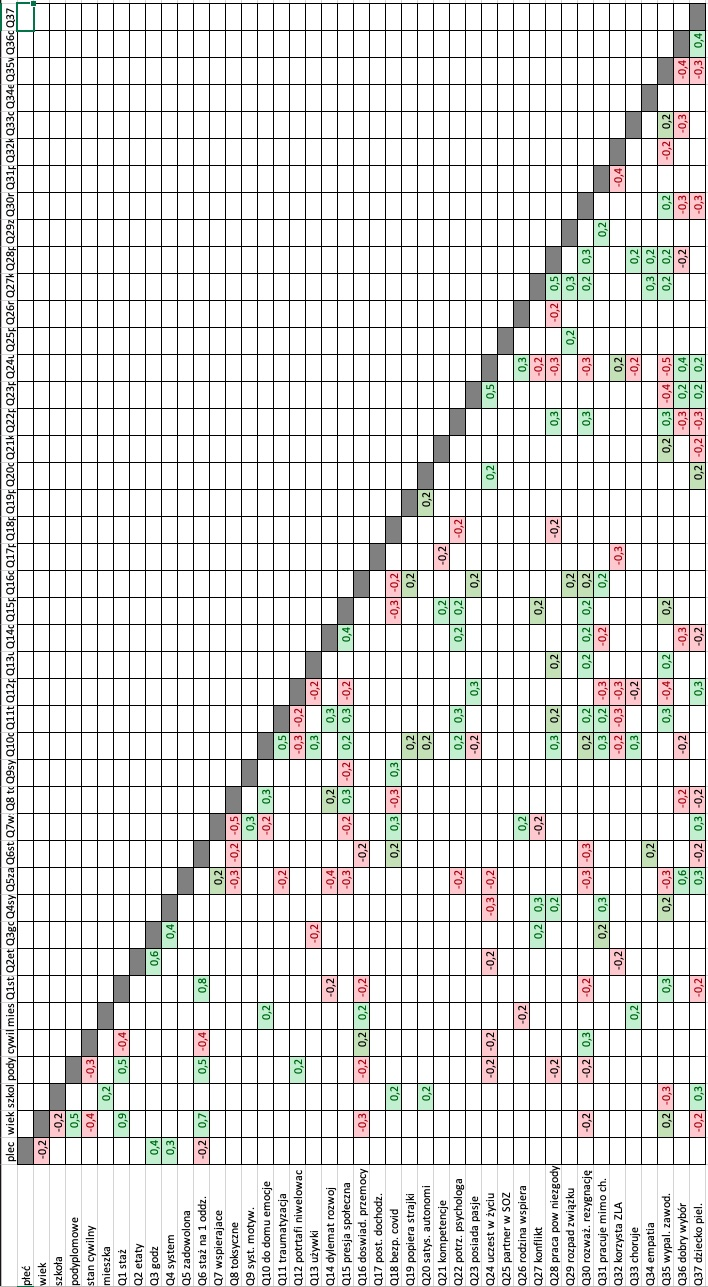
\includegraphics[width=11cm]{wyniki/crosstable90}
\caption{Tabela korelacji. Badania własne 2021/2022 r.}
\label{rys:crosstable}
\end{figure}

Przedstawiona powyżej tablica korelacji jest wynikiem wstępnej analizy statystycznej danych z ankiety. Na obu osiach oznaczono zmienne podane korelacji. Na przecięciach tych zmiennych można zaobserwować pola oznaczone kolorem i wartością liczbową. Pola te oznaczają, że pomiędzy zmiennymi zachodzi pewna korelacja. 
Wartość liczbowa określa siłę korelacji. Zakres tej siły zawiera się w przedziale od -1.0 do 1.0, przy czym wartości bliżej zera oznaczają słabszą korelację niż te bliżej bezwzględnej wartości 1. Znak liczby +/- określa kierunek korelacji. Znak dodatni, podkreślony kolorem zielonym pola, wskazuje na korelacje proporcjonalną, podczas gdy znak ujemny (kolor czerwony) oznacza korelację odwrotnie proporcjonalną.

\end{appendices}


%	\zakonczenie  % wklejenie recenzji i opinii

\end{document}
%+++ END +++



%Streszczenie
%
%Wstęp opisuje rozwój pielęgniarstwa na przestrzeni wieków, pokazując jak z prostej opieki ewoluowało do rangi dziedziny badaweczej i profesji zaufania publicznego. 
%
%Autor podejmuje próbę odpowiedzi na pytanie o cenę wykonywania tej profesji, w obliczu konieczność nieustannego rozwoju i niełatwych wyzwań, które niejednokrotnie prowadzą do deficytów w życiu osobistym i rodzinnym. 
%
%Cel niniejszej pracy to określenie wpływu pracy zawodowej na życie osobiste pielęgniarek i pielęgniarzy.
%
%W toku pracy badawczej wykorzystano metodę analizy piśmiennictwa z wykorzystaniem klasycznych technik treściowych, oraz metodę sondażu diagnostycznego z wykorzystaniem techniki ankietowej – autorskiego formularza ankiety. 
%
%Zastosowano metody statystyczne w celu analizy prezentowanych zjawisk. Badaniem objęto 115 studentów studiów niestacjonarnych na kierunku pielęgniarstwo Wyższej Szkoły Medycznej w Legnicy. Badanie przeprowadzano od 11.2021 do 02.2022.
%
%Uzyskane wyniki poddano analizie statystycznej. Wykorzystano przy tym test niezależności $\chi^2$ Pearsona.
%
%Wyniki.
%
%...
%
%
%Wnioski.
%
%
%Słowa kluczowe: pielęgniarka, praca, rodzina, satysfakcja zawodowa
%
%
%Wnioski
%Prezentowane badania mają kilka ograniczeń. W związku z tym, że ankieta była przeprowadzana on line, nie można mieć pewności, że, odpowiedzi udzielali tylko i wyłącznie studenci WSM w Legnicy.  Chociaż, kwestionariusz badań jest anonimowy, nie można wykluczyć efektu oczekiwań autora. Również osobisty charakter pytań, może powodować tendencyjność odpowiedzi. Odpowiedzi na pytania mogą się różnić w zależności od własnych doświadczeń czy obecnej sytuacji zawodowej i osobistej. Mimo tych ograniczeń, można uznać, iż wyniki badania są reprezentatywne i wnoszą istotne informacje na temat wpływu pracy zawodowej na życie osobiste pielęgniarek i położnych.
%Implikacje i kierunki kolejnych badań.
%Niniejsza praca badawcza, zwraca uwagę, na niepokojące zjawiska tj. pracę w ponadnormatywnym czasie, niekorzystanie ze zwolnień lekarskich, gdy są do tego wskazania i wykonywanie działalności zawodowej w tym czasie, stosowanie używek, czy brak poczucia bezpieczeństwa w pracy zawodowej.
%1.	 Uzyskane wyniki ewidentnie wskazują, iż pielęgniarki są obarczone pracą w ponadnormatywnym czasie. Aby zapobiegać obniżonej jakości pracy, należy wprowadzić skuteczne rozwiązania systemowe, sankcjonujące pracę w nadgodzinach. Zarządzający placówkami ochrony zdrowia powinni zmierzać do wprowadzenia odpowiednich procedur, które zapewnią bezpieczeństwo pracy personelowi i bezpieczeństwo pacjenta. (literatura)
%2.	Zarządzający zasobami ludzkimi w zakładach opieki medycznej, powinni zapewnić szkolenia i możliwości rozwoju zawodowego w zakresie komunikacji, technik psychologicznych walki ze stresem. Powinni kształtować wspierające środowisko pracy, reagując na informacje zwrotne płynące od personelu i chronić go przed traumą. Działania te muszą być zgodne z harmonogramem pracy pracownika. W sytuacji niezwykle traumatycznej dla pracownika, zespołu powinno się udzielić krótkiego urlopu, a jeśli nie jest to możliwe, zapewnić przesunięcie do pracy, która wymaga zaangażowania na innym polu.
%3.	Powinno się dążyć do pozytywnego wzmacniania personelu, stosowania systemów motywacyjnych, regularnego wspierania przez afirmację sukcesu: terapeutycznego, zawodowego i osobistego.
%4.	Powinno się do promować pielęgniarstwo jako prestiżowy zawód, zarówno lokalnie jak i globalnie w mediach, poprzez wywiady, akcje informacyjne z osobami z osiągnięciami w dziedzinie pielęgniarstwa, Powinno się podkreślać znaczenie EBM.
%5.	Powinno się dążyć, do maksymalnego wykorzystania uprawnień i kompetencji zawodowych pielęgniarek, by podnieść rangę zawodu. Należy, również skorzystać z doświadczenia zawodowego pielęgniarek z wieloletnim stażem, o wysokim poziomie satysfakcji zawodowej, a niskim poziomie wypalenia zawodowego, gdyż są cennym źródłem wiedzy o funkcjonowaniu w środowisku pracy.
%
%Implikacje te wskazują na interesujące kierunki przyszłych dociekań naukowych.
%
